\documentclass{article}

% NeurIPS 2026 style (will migrate to ICLR 2027 template before submission)
\usepackage[final]{neurips_2026}

\usepackage[utf8]{inputenc}
\usepackage[T1]{fontenc}
\usepackage{hyperref}
\usepackage{url}
\usepackage{booktabs}
\usepackage{amsfonts}
\usepackage{amsmath}
\usepackage{amssymb}
\usepackage{nicefrac}
\usepackage{microtype}
\usepackage{graphicx}
\usepackage[table]{xcolor}
\usepackage{algorithm}
\usepackage{algorithmic}
\usepackage{subcaption}
\usepackage{multirow}
\usepackage{wrapfig}

\graphicspath{{figures/}{../outputs/standard/analysis/}{../outputs/vla/}}

\newcommand{\attnres}{\textsc{AttnRes}}
\newcommand{\reskip}{\textsc{ReSkip}}
\newcommand{\reloop}{\textsc{ReLoop}}
\newcommand{\retrofit}{\textsc{AR-Retrofit}}
\newcommand{\routeA}{\textsc{Route-A}}
\newcommand{\routeB}{\textsc{Route-B}}
\newcommand{\routeC}{\textsc{Route-C}}
\newcommand{\E}{\mathbb{E}}
\newcommand{\R}{\mathbb{R}}
\newcommand{\softmax}{\text{softmax}}
\newcommand{\todo}[1]{\textcolor{red}{[TODO: #1]}}

\title{Retrofitting Pretrained Transformers for Zero-Cost\\Adaptive Computation via Attention Residuals}

\author{
  Author One\thanks{Equal contribution.} \\
  Affiliation \\
  \texttt{email@example.com} \\
  \And
  Author Two\footnotemark[1] \\
  Affiliation \\
  \texttt{email@example.com} \\
}

\begin{document}

\maketitle

\begin{abstract}
Adaptive computation promises to match transformer inference cost to input complexity, but existing methods---early exit classifiers, mixture-of-depths, layer pruning---either require auxiliary networks, from-scratch training with compute-aware losses, or irreversible post-hoc surgery that degrades quality.
We observe that \emph{Attention Residuals} (\attnres{})~\citep{chen2026attnres}---a drop-in replacement for the standard residual that attends over previous block outputs with a learned pseudo-query---already encode the routing signal adaptive computation needs, and their two-phase execution makes this signal available \emph{before} each block runs, at near-zero extra cost.
We develop this observation into a practical recipe in three parts.
\textbf{(1)~\reskip{}}: we read the phase-1 \attnres{} weights as a pre-execution skip signal, with position-calibrated thresholds. On a 340M from-scratch \attnres{} transformer, \reskip{} delivers $1.19\times$ wall-clock speedup at zero downstream degradation, and we document an \emph{importance--ablation disconnect} that makes combining router-importance and static-removal signals strictly dominant over either alone.
\textbf{(2)~\retrofit{}} (the main contribution): we convert \emph{any} pretrained transformer into an \attnres{}-capable model through a single light fine-tune---a \emph{$\gamma$-gated residual injection} that is identity-at-init, trains only small routers and adapters with the base frozen, and converges every block to $\gamma_n{=}1$ (structurally pure \attnres{}). On Qwen3-VL-2B and Qwen3-VL-4B the retrofit preserves or strictly improves base quality on text and full-set VLM benchmarks while inheriting \reskip{}'s phase-1 dynamic skip; its structural wall-clock cost is a per-block router that skip partially, but not fully, recovers.
\textbf{(3)~VLA application}: warm-starting a Qwen3-VL$+$OFT action head from the retrofit and fine-tuning on LIBERO beats a matched pure-OFT baseline at both 2B and 4B, and a control that forgoes the VLM retrofit does not close the gap even at double the VLA compute---the retrofit warm-start is not substitutable by longer VLA training.
Together, these give a path from an off-the-shelf transformer to an adaptive-depth model in a single fine-tune pass, with no architectural changes at inference.
\end{abstract}

%----------------------------------------------------------------------
\section{Introduction}
\label{sec:intro}
%----------------------------------------------------------------------

Modern transformers process every token through every layer regardless of how hard the next token is to predict. Several lines of work try to fix this mismatch: early-exit methods~\citep{schuster2022confident, elbayad2020depth} add auxiliary classifiers per layer, Mixture-of-Depths~\citep{raposo2024mixture} learns per-token routing with an auxiliary capacity loss, layer-pruning approaches~\citep{gromov2024unreasonable, men2024shortgpt} remove layers post-hoc, and Universal Transformers~\citep{dehghani2018universal} share weights across depth with explicit halting~\citep{graves2016adaptive}. All of these share a limitation: the routing signal---whether to spend more compute---is \emph{external} to the core transformer computation and must be added either as training-time supervision, a separate head, or a post-hoc heuristic.

\paragraph{Insight.}
Attention Residuals (\attnres{})~\citep{chen2026attnres} replace the fixed scalar-$1$ residual with a learned softmax attention over all previously completed block outputs. The attention weights $\alpha_{n \to l}$ are input-dependent, competitively normalised, and---crucially for this paper---are computed \emph{before} block $l$ runs, as part of forming the block's input. Two observations follow. First, the weights already constitute a natural routing signal: a block that downstream blocks never attend to is, by construction, a block that can be skipped. Second, this signal is available as a pre-execution check, at negligible cost, so we can make the skip decision \emph{at inference time}, per input, without additional parameters or training.

\paragraph{From LLMs to latency-critical VLAs.}
Our first-phase validation shows this idea works at scale: on a 340M from-scratch \attnres{} transformer pretrained on FineWeb-Edu, phase-1 skip yields $1.19\times$ wall-clock speedup at \emph{zero} benchmark degradation (Section~\ref{sec:reskip}). But the absolute latency picture sharpens as we move downstream: even block-level \attnres{} still pays a per-block phase-1 probe cost, and at the sub-10B scale that powers real-time robotics---Vision-Language-Action (VLA) systems with closed-loop control cycles of $\leq\!100$\,ms---every millisecond of per-layer overhead is visible. A VLA cannot afford a mechanism that \emph{adds} latency to buy adaptiveness; it needs a mechanism that \emph{pays for itself in speed} on average.

\paragraph{But training \attnres{} from scratch is prohibitive.}
\attnres{} is an architectural modification: the pseudo-queries $\{\mathbf{w}_l\}$ and the online-softmax merge (Algorithm~\ref{alg:two_phase}) have no counterpart in a standard residual network. Every existing \attnres{} model in the literature, including the one validated in Section~\ref{sec:reskip}, was pretrained with \attnres{} from step zero. Reproducing this at 2--7B VLM scale costs tens of thousands of GPU-hours, and in the VLA case one must further retrain the action head on top of a model with a non-standard backbone---which makes no sense when a strong open-weight standard VLM (e.g., Qwen3-VL-2B, InternVL-2.5, InternVL-3) is already available and being actively improved by the community. If adaptive-depth inference is to have practical value for latency-critical applications, we need a way to \emph{retrofit} a pretrained, standard-residual transformer into an \attnres{}-capable one---through a short, cheap fine-tune that \textbf{(i) preserves, or ideally improves, benchmark quality}, \textbf{(ii) inherits \reskip{}'s phase-1 dynamic skip so that per-input speedup offsets the introduced per-block probe cost}, and \textbf{(iii) leaves the base weights usable for the downstream action-head training that follows}.

\paragraph{Contributions.}
This paper delivers that retrofit recipe, along with its downstream application to skipping and to vision--language--action models.

\begin{enumerate}
\item \textbf{\reskip{} (Section~\ref{sec:reskip}).} We formalise the two-phase execution of \attnres{} as an implicit pre-execution routing channel and turn it into a dynamic, per-input skip rule with position-calibrated thresholds. On 340M from-scratch \attnres{} we achieve \textbf{$1.19\times$ wall-clock speedup at zero benchmark degradation}. We further identify an \emph{importance--ablation disconnect}: the \attnres{} importance score (``how often is block $n$ referenced?'') does \emph{not} align monotonically with static removal impact (``is block $n$ irreplaceable?''). Combining the two signals to pick skip candidates strictly dominates using either alone.

\item \textbf{\retrofit{} (Section~\ref{sec:retrofit}, main contribution).} We converge on a single, concrete recipe: a \emph{$\gamma$-gated block-level residual injection} that inserts \attnres{} into the pretrained forward in a provably identity-preserving way.
  \begin{itemize}
  \item Per block $n$ we add one \attnres{} router $w_n$ and a tiny residual adapter $A_n$, producing $r_n = \sum_i \alpha_{i\to n}\,h_i$ and then $x_n = h_{n-1} + \gamma_n\,A_n(r_n - h_{n-1})$; the block runs as $h_n = \mathrm{Block}_n(x_n)$.
  \item $\gamma_n$ is zero-initialised and the adapter up-projection is small-random; the retrofit at step $0$ is bit-identical to the pretrained model on downstream benchmarks.
  \item The base backbone (28 text decoder layers in our Qwen3-VL-2B target) is \emph{completely frozen}. Only the routers, adapters, and $\gamma$ train---$\sim$$15$M parameters ($\sim$$0.7\%$ of the base) at $r{=}256$.
  \item Training uses a small SFT mixture with a full-path task loss, a skip-branch consistency KL, and a light $\alpha$-entropy regulariser; $5$k--$10$k steps suffice depending on the data mix.
  \item The retrofit composes cleanly with \texttt{use\_cache=True}: on skipped blocks we still execute a K/V-only projection path (\texttt{input\_layernorm}$\to$\texttt{k\_proj/v\_proj}$\to$\texttt{k\_norm}$\to$\texttt{RoPE}$\to$\texttt{cache.update}) so generate remains length-consistent and byte-identical in argmax to the full-path cache forward (Section~\ref{sec:retrofit_cache}).
  \end{itemize}
  On Qwen3-VL-2B with a $5$k-step $\gamma{\to}1$ curriculum on a $50/50$ UltraChat+LLaVA mix (H\_r256\_5k), every block converges to $\gamma_n{=}1$ so the retrofitted model is \emph{structurally pure \attnres{}}. It takes the model from base LAMBADA acc $0.532$ to $0.576$ ($+4.4$pp / $-17$\% ppl), improves HellaSwag by $+1.6$pp, and preserves MMBench / MMStar within the $n{=}300$ noise floor. A richer $10$k-step mix anchored on LLaVA-OneVision (``v3'') further lifts every major VLM benchmark strictly above base on full \texttt{lmms-eval}: MMBench $+3.5$pp, MMMU $+2.5$pp, AI2D $+2.9$pp, OCRBench $+3.7$pp, RealWorldQA $+2.0$pp. Wall-clock on an H100 under \texttt{use\_cache=True}: the block-level router+adapter is a structural $1.37$--$1.40\times$ cost over stock Qwen3-VL-2B; phase-1 dynamic skip recovers $5$--$9\%$ on top of the retrofit-full path. \emph{The retrofit is the contribution; the skip capability comes for free from the resulting structure, and the structural cost is the scalar we characterise throughout.}

\item \textbf{VLA application (Section~\ref{sec:vla}).} We warm-start a Qwen3-VL-2B OFT policy from the retrofit state and fine-tune on LIBERO-90~\citep{liu2023libero}. The retrofit warm-start (``Path B'') reaches $97.15\%$ 4-suite average success on 2B (reporting Path B's per-suite max and Path 0's per-suite min over the two seeds we ran, see Section~\ref{sec:vla_variance}), $+1.30$pp above a pure-OFT baseline trained for the same $30$k steps; the same recipe on a clean Qwen3-VL-4B reaches $96.70\%$ single-run ($+0.65$pp vs.\ its matched 4B baseline). A $\gamma$-curriculum control that skips the VLM retrofit (``Path C'') plateaus at $94.30\%$ at $30$k steps and only $95.50\%$ at $60$k: \emph{the VLM retrofit warm-start is not substitutable by longer VLA training.} We also identify a concrete pipeline hazard---unfrozen action-token embeddings in an ``Instruct-Action'' base leak gradient into the shared \texttt{lm\_head} and drop \texttt{libero\_10} by $9.4$pp.
\end{enumerate}

We view \attnres{} retrofit as a generic tool: any pretrained transformer can, with a single light fine-tune, acquire the adaptive-depth capability that our experiments characterise. Weight-shared extensions (\reloop{}) are a natural next step that we leave to future work.

%----------------------------------------------------------------------
\section{The Latency Problem \attnres{} Must Solve}
\label{sec:motivation}
%----------------------------------------------------------------------

The promise of \attnres{} is \emph{adaptive depth at no extra serving cost}: blocks the model does not need are skipped, and the skip decision reuses a quantity the model was going to compute anyway (the phase-1 weight). This section reports what actually happens on the clock---both at the 340M scale where \attnres{} was first validated and at the 2B VL scale that matters for the downstream robotics setting---and uses those numbers to argue that the retrofit path developed in Sections~\ref{sec:retrofit}--\ref{sec:vla} is necessary.

\subsection{\attnres{} is not free: block-level probe overhead at 340M}
\label{sec:motivation_latency}

We measure forward-pass latency on 1$\times$H100, bfloat16, batch$=$1, random-token inputs (5 warmup + 20 timed passes, median) for two models trained under identical FineWeb-Edu 100BT recipe at 340M parameters: a \textbf{vanilla standard-residual transformer}, and an \textbf{\attnres{} transformer} pretrained from scratch with block-\attnres{} ($N=8$ blocks).

\begin{table}[t]
\caption{Forward-pass wall-clock at 340M scale (H100, bfloat16, batch 1, random tokens, median of 20 runs). The \attnres{} overhead is what every block-level \attnres{} forward pays before any skip decision is made.}
\label{tab:motivation_340m_latency}
\centering\small
\begin{tabular}{ccc|c}
\toprule
seq & vanilla 340M & \attnres{} 340M (block-\attnres{}) & $\Delta$ \attnres{} vs vanilla \\
\midrule
512   & 14.0\,ms & 31.3\,ms & $+$123\,\% \\
1024  & 13.7\,ms & 31.1\,ms & $+$128\,\% \\
2048  & 14.0\,ms & 31.6\,ms & $+$126\,\% \\
8192  & 25.7\,ms & 45.8\,ms & $+$78\,\% \\
\bottomrule
\end{tabular}
\end{table}

\paragraph{Reading the table.}
\textbf{\attnres{} is measurably slower than a matched vanilla transformer}, by a factor large enough to swamp the inference budget at small scale and short sequence length. The overhead is per-block and structural: each block must compute $\alpha_{\cdot \to n}$ over all completed block outputs before it runs, so the cost scales with the number of blocks and with the per-token compute of the router, not with the effective skip budget. The relative overhead shrinks at long sequences because attention cost grows super-linearly, but in \emph{absolute} milliseconds it remains $\geq 15$\,ms across every seq we measured: on a $\sim$14\,ms vanilla baseline, that is more than doubling the per-forward cost of the model.

This cost is paid \emph{before} any runtime adaptiveness is applied. Whether it can be paid back---by skipping enough blocks on enough inputs to net out favourably---is a second question that we take up in Sections~\ref{sec:reskip}--\ref{sec:retrofit}; for now, the point is that ``add \attnres{}'' is not a free architectural swap, and it is least free at the scale and sequence regime that downstream latency-critical applications actually target.

\subsection{Why this is a load-bearing constraint for VLA}
\label{sec:motivation_vla}

Robotic closed-loop control imposes a hard real-time budget. Representative targets from recent open VLA work~\citep{black2024pi0, kim2024openvla}: Pi0 runs a 50\,Hz low-level controller ($20$\,ms per cycle) on top of a language-conditioned high-level policy; OpenVLA-7B reports approximately 6\,Hz ($\sim$166\,ms per cycle) at bfloat16 on a single GPU. General manipulation benchmarks target 10--50\,Hz (20--100\,ms budgets). Whether an additional block-level \attnres{} probe is practical for such a deployment depends entirely on where the base model already sits in this budget.

Table~\ref{tab:motivation_vlm_latency} reports stock Qwen3-VL-2B latency at the sequence lengths that VLA systems actually use (short instruction only; instruction + one visual frame; instruction + image + short context; multi-turn dialogue with images; long-horizon trajectory context).

\begin{table}[t]
\caption{Stock Qwen3-VL-2B forward-pass latency (H100, bfloat16, batch 1, single image where applicable). The ``what it represents'' column maps sequence length to VLA usage.}
\label{tab:motivation_vlm_latency}
\centering\small
\begin{tabular}{cllcc}
\toprule
seq & representative VLA usage & control-rate budget & stock Qwen3-VL-2B latency \\
\midrule
256  & pure short instruction                   & 50\,Hz $\leq 20$\,ms      & 25.6\,ms \\
512  & instruction + 1 image (tokenised)        & 20\,Hz $\leq 50$\,ms      & 23.3\,ms \\
1024 & instruction + image + short context      & 10\,Hz $\leq 100$\,ms     & 23.8\,ms \\
2048 & multi-turn dialogue w/ images            & 5\,Hz $\leq 200$\,ms      & 33.9\,ms \\
4096 & long-horizon trajectory context          & 2--5\,Hz                 & 77.1\,ms \\
\bottomrule
\end{tabular}
\end{table}

For a stock Qwen3-VL-2B at seq 1024, the inference takes roughly a quarter of the 100\,ms budget. A 35--45\,\% block-level \attnres{} overhead (Table~\ref{tab:motivation_340m_latency}) would push that past the 10\,Hz line and into the territory where adaptive-depth is a liability rather than an asset. Conversely, a retrofit that (a) leaves the base unchanged and (b) recovers the probe overhead through skip savings keeps us under budget while gaining input-dependent compute---exactly the balance Section~\ref{sec:retrofit} aims for.

\subsection{From-scratch \attnres{} at VLA scale is prohibitive}
\label{sec:motivation_cost}

Sections~\ref{sec:motivation_latency} and~\ref{sec:motivation_vla} say that if we were handed a 2B \attnres{}-pretrained VLM, it would already be fighting the VLA latency budget. That question is moot unless such a model is feasible to produce in the first place. To calibrate what ``produce it'' would cost, Table~\ref{tab:motivation_cost} collects published training-compute numbers for recent open VLMs and VLAs at the 2--7B scale. The lower bound of what we would have to pay for a 2B \attnres{}-VLM is whatever the \emph{standard} open models at that scale already cost; \attnres{} is never cheaper than the pretrain it replaces.

\begin{table}[t]
\caption{Published training scales for recent open VLMs and VLAs at the 0.5--7B class. Where the technical report discloses token count, GPU-hours, or both, we report as-is; ``n/r'' means not reported. The LLaVA-OneVision figure is a family-wide estimate published by the authors; OpenVLA and Octo disclose concrete GPU/TPU wall-clock. The bottom row is a lower-bound extrapolation: pretraining a 2B \attnres{}-VLM from scratch cannot take less compute than the same-scale standard-residual models above, and block-level \attnres{} adds further per-step overhead (Table~\ref{tab:motivation_340m_latency}).}
\label{tab:motivation_cost}
\centering\small
\begin{tabular}{lcclll}
\toprule
system & scale & modality & training data & GPU-hours reported & reference \\
\midrule
Qwen3-VL-2B              & 2\,B    & VLM & ${\sim}2.2$\,T tokens     & n/r                  & \citep{bai2025qwen3vl} \\
InternVL3-2B             & 2\,B    & VLM & ${\sim}200$\,B tokens     & n/r                  & \citep{zhu2025internvl3} \\
LLaVA-OneVision          & 0.5--7\,B & VLM & 1.6\,M multimodal samples & ${\sim}26.7$k A100-h (est.) & \citep{li2024llavaonevision} \\
OpenVLA                  & 7\,B    & VLA & 970k robot trajectories   & 64$\times$A100 $\times$ 14\,d $= 21.5$k A100-h & \citep{kim2024openvla} \\
$\pi_0$                  & 3.3\,B  & VLA & 10k+\,hr robot + OXE      & n/r                  & \citep{black2024pi0} \\
Octo-B                   & 0.09\,B & VLA & 800k trajectories (OXE)   & 128$\times$TPUv4 $\times$ 14\,h $= 1.8$k TPU-h & \citep{team2024octo} \\
\midrule
\textbf{2B \attnres{}-VLM pretrain (implied)} & 2\,B & VLM & $\geq$ Qwen3-VL-2B / InternVL3-2B & $\geq$ same, $+$block-\attnres{} overhead & this work \\
\bottomrule
\end{tabular}
\end{table}

Two readings of the table:
\emph{(i)} Standard 2B-class VLM pretraining budgets are already large (the order of magnitude that groups can afford only at the model-release level, not at the method-paper level). Reproducing a single one of these runs to swap the residual connection for \attnres{} is not an experiment an academic lab or deployment team will volunteer to run.
\emph{(ii)} VLA systems inherit this cost and then add training data of their own---OpenVLA, $\pi_0$, Octo are all post-trained on top of already-pretrained backbones, not trained end-to-end from scratch, precisely because the standard-residual backbones they start from are the only artifacts at that scale that exist.

The cost asymmetry is the reason this paper exists. If \attnres{} is going to be used beyond the controlled 340M FineWeb-Edu setting that produced it (Section~\ref{sec:reskip}), the access path cannot be ``retrain from scratch.'' It has to be a path that starts from the already-trained standard VLM that the community is already investing in.

\subsection{Summary: the gap a solution has to close}
\label{sec:motivation_gap}

Together, Sections~\ref{sec:motivation_latency}--\ref{sec:motivation_cost} characterise a non-trivial gap:

\begin{itemize}
  \item \textbf{(Latency, intrinsic)} Block-level \attnres{}, pretrained as intended, costs measurable wall-clock over a matched standard transformer (Table~\ref{tab:motivation_340m_latency}). Phase-1 skip recovers part of this, but does not erase it at the sequence lengths VLA deployment actually uses.
  \item \textbf{(Deployment budget)} At the 2B scale where a VLA backbone sits, the per-forward budget imposed by 10--50\,Hz control (Table~\ref{tab:motivation_vlm_latency}) leaves little headroom for uncovered \attnres{} overhead.
  \item \textbf{(Access)} There is no shortcut. Either the community spends 10{,}000--25{,}000 H100-hours pretraining a 2B \attnres{}-VLM (Table~\ref{tab:motivation_cost}), or \attnres{} as an inference-time capability is unavailable to the VLA setting at all.
\end{itemize}

Any solution has to close \emph{both} ends: it has to make \attnres{} installable on an already-pretrained standard VLM without rerunning pretraining, and it has to install it in a way whose runtime cost---including the block-level probes and any additional machinery it introduces---is at worst neutral, ideally favourable, with respect to the stock base. Sections~\ref{sec:background}--\ref{sec:retrofit} develop and Section~\ref{sec:experiments} tests such a solution.

%----------------------------------------------------------------------
\section{Background: Attention Residuals}
\label{sec:background}
%----------------------------------------------------------------------

\subsection{Standard residual connections}
In a standard transformer with $L$ layers,
\begin{equation}
  \mathbf{x}_l = \mathbf{x}_{l-1} + f_l(\mathbf{x}_{l-1}), \qquad
  \mathbf{x}_L = \mathbf{x}_0 + \sum_{l=1}^{L} f_l(\mathbf{x}_{l-1}).
\end{equation}
The combination weights are fixed at $1$ for every layer and every input---no routing information is emitted.

\subsection{Attention Residuals}
\attnres{}~\citep{chen2026attnres} replaces the fixed combination with a learned attention over depth. Each block $l$ maintains a pseudo-query $\mathbf{w}_l \in \R^d$; keys are projections $\mathbf{k}_i = W_K \mathbf{h}_i$ of earlier block outputs $\mathbf{h}_i$:
\begin{equation}
  \alpha_{i \to l} = \frac{\exp(\mathbf{w}_l^\top \mathbf{k}_i / \sqrt{d})}{\sum_{j=0}^{l-1} \exp(\mathbf{w}_l^\top \mathbf{k}_j / \sqrt{d})},
  \qquad
  \mathbf{x}_l = \sum_{i=0}^{l-1} \alpha_{i \to l}\,\mathbf{h}_i.
  \label{eq:attnres}
\end{equation}
For efficiency, block-\attnres{} groups layers into $N$ blocks and applies the softmax at the block level, which is the granularity we use throughout.

\paragraph{Two-phase execution.}
A subtle but crucial property: computing the input to block $l$ requires only $\{\mathbf{h}_i\}_{i<l}$ and $\mathbf{w}_l$, both of which are available \emph{before} block $l$ runs. We refer to this as \emph{phase~1} (pre-execution attention over completed blocks). \emph{Phase~2} is the block's own transformation $f_l$; its output is folded into the running online-softmax state to produce the input of the next block. Algorithm~\ref{alg:two_phase} presents the unified two-phase forward, with \reskip{}'s dynamic skip check introduced at line~6.

\begin{algorithm}[t]
\caption{Two-phase \attnres{} forward with dynamic \reskip{}}
\label{alg:two_phase}
\begin{algorithmic}[1]
\STATE \textbf{Input:} Embeddings $\mathbf{h}_0$; block functions $f_1, \ldots, f_N$; pseudo-queries $\{\mathbf{w}_n\}$; eligible positions $\mathcal{P}$; thresholds $\{\tau_n\}_{n\in\mathcal{P}}$; max skips $M_{\max}$.
\STATE Initialise online-softmax state $(\mathbf{s}, m, e) \gets \textsc{Init}(\mathbf{h}_0)$; skip counter $k \gets 0$.
\FOR{$n = 1$ to $N$}
  \STATE \textbf{Phase 1 (probe).} Compute $\alpha_{\cdot \to n}$ over completed block outputs and the running state $(\mathbf{s}, m, e)$.
  \STATE Extract $w_{\text{recent}}(n) \gets \E_{\text{token}}[\alpha_{n-1 \to n}]$.
  \IF{$n \in \mathcal{P}$ \textbf{and} $k < M_{\max}$ \textbf{and} $w_{\text{recent}}(n) > \tau_n$}
    \STATE \textbf{Skip} block $n$; keep state unchanged, set $\mathbf{h}_n \gets \mathbf{h}_{n-1}$, $k \gets k+1$.
  \ELSE
    \STATE \textbf{Execute} block $n$ on the phase-1 merged input; update $(\mathbf{s}, m, e)$ with the new output $\mathbf{h}_n$.
  \ENDIF
\ENDFOR
\STATE \textbf{Output:} final hidden state $\mathbf{s}/e$.
\end{algorithmic}
\end{algorithm}

%----------------------------------------------------------------------
\section{\reskip{}: AttnRes-Guided Layer Skipping}
\label{sec:reskip}
%----------------------------------------------------------------------

\reskip{} turns the phase-1 signal of \attnres{} into a per-input skip rule. We first describe the method (Section~\ref{sec:reskip_method}), then expose a finding about block-level importance that informs eligible-position selection (Section~\ref{sec:reskip_disconnect}), and finally validate the approach on a 340M from-scratch \attnres{} model (Section~\ref{sec:reskip_results}).

\subsection{Method}
\label{sec:reskip_method}

\paragraph{Two offline scores per block.}
We characterise each block~$n$ with two complementary quantities computed on a small calibration set:
\begin{align}
I(n) &= \max_{l > n}\,\E\!\left[\alpha_{n \to l}\right]
  && \text{(\emph{\attnres{} importance}: how often block $n$ is referenced)} \label{eq:importance} \\
A(n) &= \frac{\text{PPL}(\text{model with block $n$ statically removed})}{\text{PPL}(\text{full-depth})}
  && \text{(\emph{ablation impact}: is block $n$ irreplaceable?)} \label{eq:ablation}
\end{align}
$I(n)$ requires only forward passes; $A(n)$ requires $N-2$ ablated forward passes. Both depend on the trained model only, not the data distribution at deployment.

\paragraph{Dynamic skip from phase-1 statistics.}
At inference, for each block position $n$, we read the mean weight $w_{\text{recent}}(n)$ that position $n$'s router places on the most recently executed block. The default skip rule \texttt{recent\_weight\_gt} is:
\begin{equation}
  \text{skip block $n$} \iff
  w_{\text{recent}}(n) > \tau_n
  \;\;\text{and}\;\;
  n \in \mathcal{P}
  \;\;\text{and}\;\;
  \textstyle\sum_{m<n} \mathbb{1}[\text{skipped}_m] < M_{\max}.
  \label{eq:skip_rule}
\end{equation}
The intuition is causal: if the next router already wants to copy the most recent output, block $n$ is doing local refinement that the model does not rely on.

\paragraph{Position-specific calibrated thresholds.}
A single global $\tau$ is sub-optimal; the distribution of $w_{\text{recent}}(n)$ differs sharply across positions. We calibrate per position on $32$ held-out long-context sequences, setting $\tau_n$ to the $q$-th empirical quantile of $w_{\text{recent}}(n)$ ($q{=}0.85$ by default). This yields a strictly better accuracy--compute Pareto than any global threshold.

\paragraph{Eligible-position selection uses both $I$ and $A$.}
Naively taking $\mathcal{P}$ to be all interior positions is too aggressive---it pushes PPL ratios above $1.3$ even at mild quantiles (Figure~\ref{fig:reskip_pareto}). Prior analyses tend to pick $\mathcal{P}$ by low $I$ alone; we show (Section~\ref{sec:reskip_disconnect}) that one must combine both scores:
\begin{itemize}
  \item \textbf{Low $I(n)$} $\Rightarrow$ skip triggers \emph{frequently} (the next router genuinely rarely uses block $n$);
  \item \textbf{Low $A(n)$} $\Rightarrow$ skip is \emph{safe} (even a mis-trigger preserves quality).
\end{itemize}

\paragraph{Cost of the skip decision.}
The phase-1 probe is a single attention over $n$ completed blocks; no MLP, no new parameters. The decision rule is a scalar comparison. Calibration produces $\tau_n$ in a single 32-batch pass and is embedded in the checkpoint's \texttt{config.json}; downstream users simply load and run. No architectural changes, no additional parameters, no training modifications.

\paragraph{Comparison to existing methods.}
Table~\ref{tab:method_comparison} summarises the differences. \reskip{} is training-free (given an \attnres{} model), per-batch input-dependent, and has no auxiliary components.

\begin{table}[t]
\caption{\reskip{} versus representative adaptive-computation methods.}
\label{tab:method_comparison}
\centering\small
\begin{tabular}{lcccc}
\toprule
Method & Auxiliary network & Routing is & Train-time changes & Architectural changes \\
\midrule
CALM~\citep{schuster2022confident} & exit classifiers & per-token & yes & small \\
Mixture-of-Depths~\citep{raposo2024mixture} & router & per-token & yes, capacity loss & yes \\
Static pruning~\citep{gromov2024unreasonable} & none & static & no & block removed \\
LayerSkip~\citep{elhoushi2024layerskip} & spec.\ decoder & per-token & yes, cont.\ pretrain & decoding path \\
\textbf{\reskip{} (ours)} & \textbf{none} & \textbf{per-batch} & \textbf{none} & \textbf{none} \\
\bottomrule
\end{tabular}
\end{table}

\subsection{The importance--ablation disconnect}
\label{sec:reskip_disconnect}

\begin{figure}[t]
  \centering
  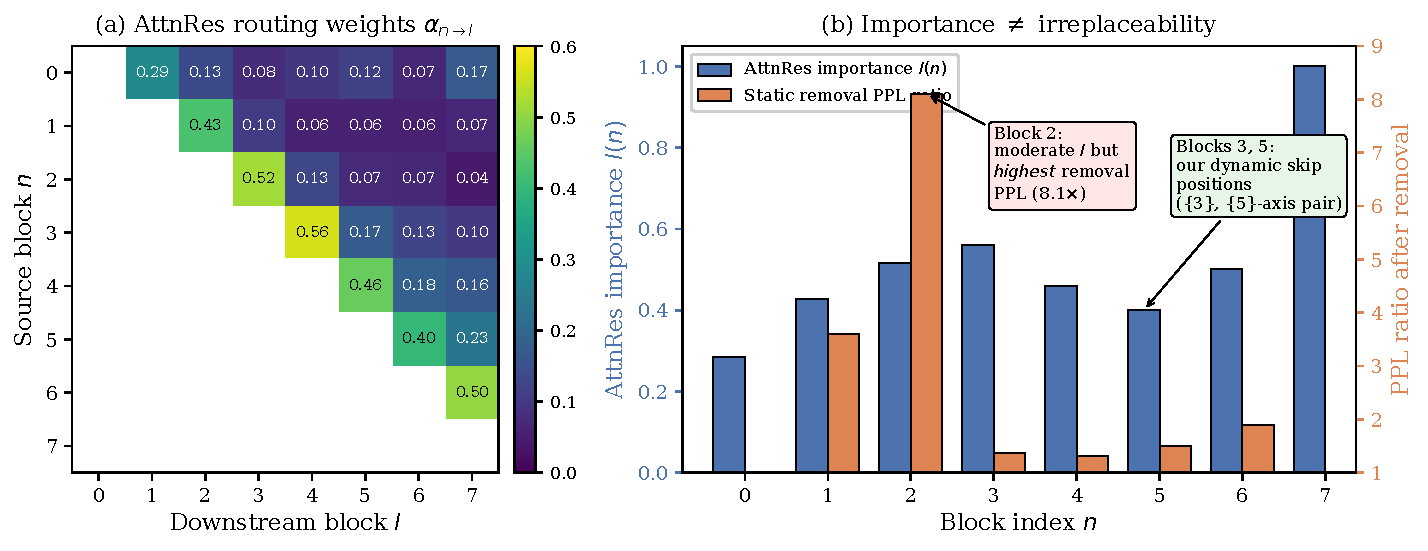
\includegraphics[width=\textwidth]{reskip_routing_importance_vs_ablation.pdf}
  \caption{\textbf{\attnres{} routing weights do not predict ablation impact (340M).} (a)~Learned block-level attention $\alpha_{n \to l}$. (b)~Per-block \emph{\attnres{} importance} $I(n)$ (blue, left axis) and \emph{static removal PPL ratio} $A(n)$ (orange, right axis). Block~2 has moderate $I$ yet the highest removal impact ($8.1\times$ PPL); blocks~3--5 span the space of low ablation impact but with very different importance levels. \reskip{} needs \emph{both} signals: low $I$ to trigger often and low $A$ to trigger safely.}
  \label{fig:reskip_routing}
\end{figure}

Figure~\ref{fig:reskip_routing} visualises the learned \attnres{} weights on our 340M model. Most attention concentrates on the immediate predecessor (diagonal band) with sparse long-range attention to the embedding and the final block---consistent with prior observations~\citep{chen2026attnres}.

\begin{wraptable}{r}{0.43\textwidth}
\vspace{-2pt}
\centering\small
\caption{Dynamic skip as a function of the candidate position set $\mathcal{P}$ on 340M ($M_{\max}{=}2$, $q{=}0.85$).}
\label{tab:reskip_position_ablation}
\begin{tabular}{lcc}
\toprule
$\mathcal{P}$ & PPL ratio & Speedup \\
\midrule
$\{5\}$ ($I$-only) & 0.993 & 1.14$\times$ \\
$\{3\}$ ($A$-only) & 1.009 & 1.02$\times$ \\
$\{2,3\}$ & 1.009 & 1.17$\times$ \\
$\{4,5\}$ & 1.008 & 0.97$\times$ \\
$\{3,4,5\}$ & 0.993 & 1.02$\times$ \\
$\{2,3,4,5,6\}$ & 1.40 & 1.16$\times$ \\
\midrule
\textbf{$\{3,5\}$ (ours)} & \textbf{0.991} & \textbf{1.19$\times$} \\
\bottomrule
\end{tabular}
\vspace{-8pt}
\end{wraptable}

The striking observation is that $I(n)$ and $A(n)$ \emph{disagree on a case-by-case basis}. Block~2 has middle-of-the-pack importance ($I{=}0.52$) yet is \emph{catastrophic} to remove ($A{=}8.1\times$). Block~4 has the lowest ablation impact ($A{=}1.31\times$) yet higher importance than block~5. The most effective dynamic-skip candidates score well on \emph{both} axes: block~5 (lowest $I$, moderate $A$) and block~3 (moderately high $I$ but low $A$).

Table~\ref{tab:reskip_position_ablation} quantifies this on the 340M model. Using block~5 alone (the low-$I$ choice favoured by prior analyses) gives $1.14\times$. Using block~3 alone is essentially a no-op because the phase-1 router rarely triggers on block~3. Combining them into $\mathcal{P}=\{3,5\}$ with $M_{\max}{=}2$ is strictly better: $1.19\times$ speedup with PPL slightly below full-depth on our proxy set.

\subsection{Results on 340M from-scratch \attnres{}}
\label{sec:reskip_results}

\paragraph{Setup.}
Block-\attnres{} transformer with $d{=}1024$, $L{=}24$ layers grouped into $N{=}8$ blocks ($\sim$340M parameters), pretrained on FineWeb-Edu~100BT~\citep{penedo2024fineweb} for 35k steps at sequence length 32k. Calibration uses 32 held-out sequences of length 8192. Wall-clock is measured on a single H100 (48 cached sequences, 4 warmup). We report \texttt{lm-eval-harness}~\citep{eval-harness} results on LAMBADA~\citep{paperno2016lambada}, HellaSwag~\citep{zellers2019hellaswag}, ARC-Easy and ARC-Challenge~\citep{clark2018arc}.

\begin{table}[t]
\caption{Downstream benchmark comparison on 340M FineWeb-Edu. Dynamic \reskip{} preserves every metric while running $1.19\times$ faster end-to-end at sequence length 8192.}
\label{tab:reskip_benchmark}
\centering\small
\begin{tabular}{lccccc}
\toprule
\textbf{Configuration} & \textbf{LAMBADA acc} & \textbf{LAMBADA ppl} & \textbf{HellaSwag} & \textbf{ARC-E} & \textbf{ARC-C} \\
\midrule
Full-depth & 0.4056 & 20.20 & 0.4607 & 0.5438 & 0.3012 \\
\reskip{} ($\mathcal{P}{=}\{5\}, M_{\max}{=}1, q{=}0.95$) & \textbf{0.4056} & \textbf{20.20} & \textbf{0.4607} & \textbf{0.5438} & \textbf{0.3012} \\
\reskip{} ($\mathcal{P}{=}\{3,5\}, M_{\max}{=}2, q{=}0.85$) & \textbf{0.4056} & \textbf{20.20} & \textbf{0.4607} & \textbf{0.5438} & \textbf{0.3012} \\
\bottomrule
\end{tabular}
\end{table}

\begin{figure}[t]
  \centering
  \begin{subfigure}[b]{0.55\textwidth}
    \centering
    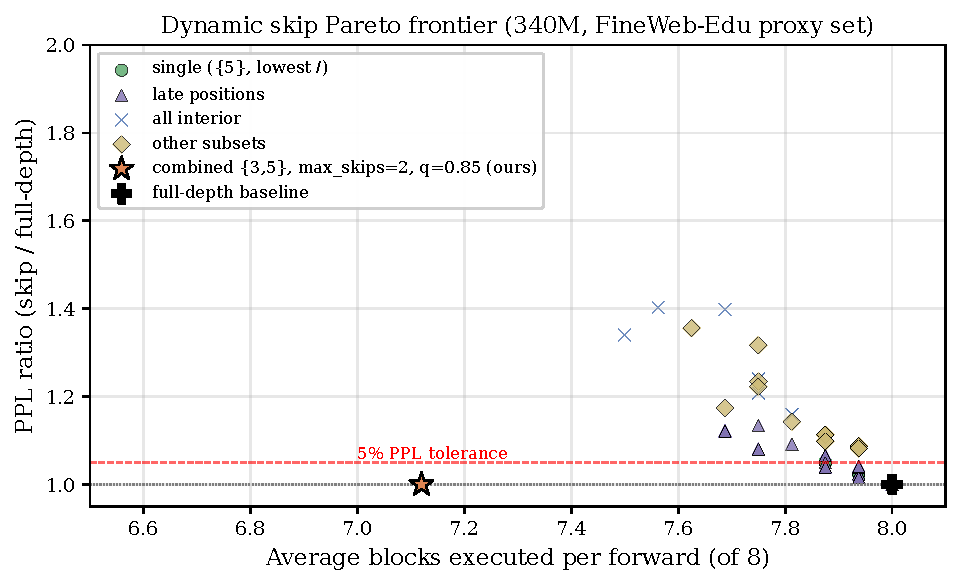
\includegraphics[width=\textwidth]{reskip_pareto.pdf}
    \caption{Accuracy--compute Pareto. $\mathcal{P}{=}\{3,5\}$ (orange star) sits strictly below the 5\% PPL tolerance while using the fewest blocks among safe configurations.}
    \label{fig:reskip_pareto}
  \end{subfigure}
  \hfill
  \begin{subfigure}[b]{0.42\textwidth}
    \centering
    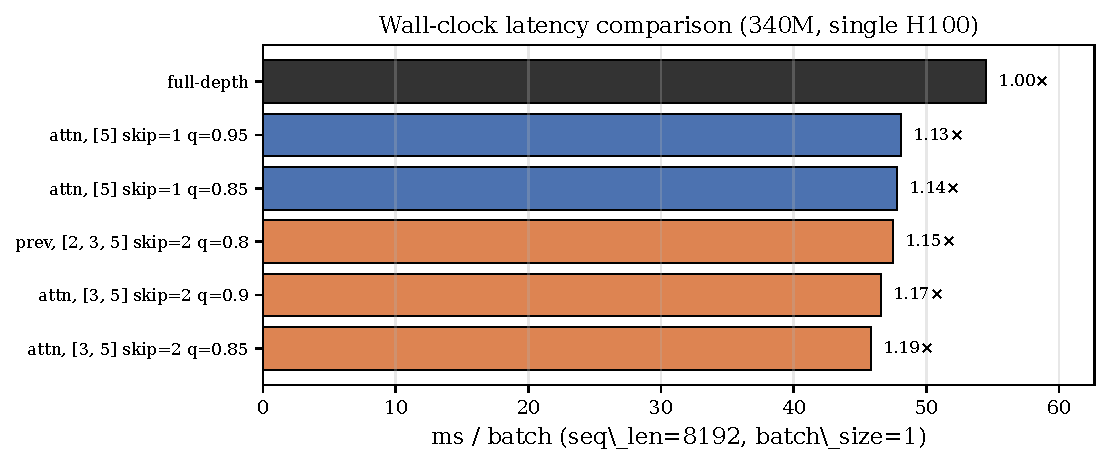
\includegraphics[width=\textwidth]{reskip_latency.pdf}
    \caption{Wall-clock latency on a single H100 at seq\_len=8192. Moving from $\{5\}/M_{\max}{=}1$ to $\{3,5\}/M_{\max}{=}2$ improves speedup from $1.14\times$ to $1.19\times$.}
    \label{fig:reskip_latency}
  \end{subfigure}
  \caption{\reskip{} on 340M FineWeb-Edu. Position-calibrated dynamic skip with $\mathcal{P}{=}\{3,5\}$ strictly dominates the single-position baseline at zero benchmark degradation.}
  \label{fig:reskip_pareto_latency}
\end{figure}

\paragraph{Quality.}
Table~\ref{tab:reskip_benchmark} shows that both the single-position and combined-position configurations preserve every benchmark metric exactly. Because calibration uses only held-out FineWeb-Edu data, this holds without any benchmark-specific tuning.

\paragraph{Speed.}
Figure~\ref{fig:reskip_latency} compares six configurations measured in the same session on a single H100 with sequence length 8192. Our combined $\{3,5\}/M_{\max}{=}2/q{=}0.85$ configuration reaches $1.19\times$ over full-depth, up from $1.14\times$ when restricted to the $\{5\}$ position. Figure~\ref{fig:reskip_pareto} places this on the full Pareto frontier: no other configuration from a 90-point sweep of $(\mathcal{P}, M_{\max}, q)$ reaches the same compute ratio without exceeding the 5\% PPL tolerance.

\paragraph{Input dependence.}
Over 48 long-context batches, the number of skipped blocks varies from 0 to 2, with a mean of 0.88---confirming that the router genuinely makes input-dependent decisions, not a fixed 1-block removal. Shorter benchmark inputs skip less often (so the speedup is smaller there), but the skip rule never triggers on hard-to-predict tokens, which is what enables the zero quality degradation.

\paragraph{Validation, not contribution.}
We emphasise that Section~\ref{sec:reskip} \emph{establishes that the mechanism works} when \attnres{} is trained in. The harder question---\emph{how to acquire \attnres{} capability in an existing model}---is the subject of Section~\ref{sec:retrofit}.

%----------------------------------------------------------------------
\section{\retrofit{}: Retrofit Method}
\label{sec:retrofit}
%----------------------------------------------------------------------

\subsection{Problem statement}
Let $\theta^\star$ be the parameters of a transformer pretrained in the standard-residual regime, reaching some quality level $Q_0$ on a benchmark suite. We want to produce parameters $\theta'$ of an \attnres{} model such that:
\begin{description}
  \item[(P1)~\emph{Quality preservation:}] the retrofit model matches $\theta^\star$'s benchmark quality to within a small tolerance (we target $\leq 2\%$ mean drop).
  \item[(P2)~\emph{Routing informativeness:}] the learned pseudo-queries $\{\mathbf{w}_l\}$ produce an $\alpha$ distribution that is informative enough to drive a non-trivial \reskip{} Pareto (e.g., $\geq 20\%$ compute saved at $\leq 5\%$ PPL drop).
  \item[(P3)~\emph{Cheap:}] the fine-tune cost is small compared to pretraining, and uses off-the-shelf data.
\end{description}

\paragraph{Why this is not trivial.}
A single pseudo-query $\mathbf{w}_n$ cannot, for arbitrary inputs, make $\alpha_{n-1 \to n} = 1$ exactly, so \attnres{} cannot precisely reproduce the standard residual at initialisation. Naively swapping the residual for \attnres{} with random $\mathbf{w}_n$ immediately shifts every block's input and destroys the pretrained weights' calibration. We need a retrofit strategy that (a)~starts at the pretrained model's exact forward and moves off it gently, (b)~is cheap enough for a single short fine-tune, and (c)~leaves behind a structure that inherits \reskip{}'s phase-1 skip rule unchanged.

\subsection{The $\gamma$-gated residual-injection method}
\label{sec:retrofit_method}

We organise the $L$ decoder layers of the pretrained model into $N$ \emph{blocks} of $L/N$ layers each (in our Qwen3-VL-2B target, $L{=}28$, $N{=}14$). Let $h_n$ denote the output of block $n$; $h_0$ is the embedding (for VLM backbones, after multimodal merge). For every block $n\ge 1$ we add three new components with a combined parameter count of $\sim$\texttt{2d}~+~\texttt{2dr}~+~1 per block (router $+$ adapter $+$ gate):
\begin{equation}
  r_n = \sum_{i=0}^{n-1} \alpha_{i \to n}\,h_i
      = \sum_{i=0}^{n-1} \frac{\exp(\mathbf{w}_n^\top (\mathrm{RMSNorm}(h_i){+}\mathbf{p}_i) / \sqrt{d}\,\tau)}{\sum_j \exp(\cdot)}\,h_i ,
  \qquad
  x_n = h_{n-1} + \underbrace{\gamma_n}_{\in\mathbb{R}}\,\underbrace{A_n(r_n - h_{n-1})}_{\text{residual correction}} ,
  \qquad
  h_n = \mathrm{Block}_n(x_n).
  \label{eq:gamma_gate}
\end{equation}
Here $\mathbf{w}_n\in\mathbb{R}^d$ is the pseudo-query, $\mathbf{p}_i\in\mathbb{R}^d$ is an optional per-position key bias, $\tau$ is a fixed temperature, and $A_n\colon\mathbb{R}^d\to\mathbb{R}^d$ is a tiny two-layer bottleneck (down-project to rank $r$, SiLU, up-project) shared across tokens within a block. The standard residual within each block (attention/MLP sub-residuals) is left \emph{entirely untouched}: $\mathrm{Block}_n$ is the pretrained block, verbatim. \attnres{} enters only \emph{between} blocks, as a correction to the block-input $x_n$.

\paragraph{Identity at initialisation.}
With $\gamma_n{=}0$ we have $x_n = h_{n-1}$ regardless of what the router outputs, so the forward is bit-identical to the pretrained model. This gives us P1 for free. A subtle point: initialising both $\gamma_n{=}0$ and $A_n$'s up-projection to zero causes a gradient deadlock (the only paths to $\gamma$, $A_n$, and $\mathbf{w}_n$ all vanish). We therefore keep $\gamma_n{=}0$ but initialise $A_n$'s up-projection with small Gaussian noise (std~$0.02$); the product $\gamma_n \cdot A_n(\cdot) = 0$ still holds exactly, but $\partial \mathcal{L}/\partial \gamma_n \propto A_n(r_n-h_{n-1}) \ne 0$, so training starts with live gradients.

\paragraph{Why gate-and-adapt instead of the pure paper-proposed routes.}
Early pilots on Qwen3-VL-2B (Appendix~\ref{app:route_ablations}) tried three cleaner alternatives: (i)~\emph{observer-only}, keep the forward standard and train a distilled $\alpha$ head; (ii)~\emph{interpolation at block-input}, $x_n=(1{-}\beta_n)h_{n-1}+\beta_n r_n$ with $\beta_n$ driven to~1; (iii)~\emph{informed-init + temperature anneal} from a residual-like init. Observer-only produced an $\alpha$ signal whose skip decision \emph{does not feed back into the forward}, so on LAMBADA it collapsed to $0.12$ accuracy ($-75\%$ vs.\ base); interpolation driven to $\beta{=}1$ forced the pretrained backbone to consume an OOD input distribution ($r_n$) and required backbone updates plus pretraining data to stay afloat; informed-init suffered from near-equal pretrained keys at adjacent blocks, making the sharpness knob useless. The $\gamma$-gated residual-injection in Eq.~\ref{eq:gamma_gate} instead enters \attnres{} \emph{additively on top of} the standard residual path: the backbone keeps receiving the in-distribution $h_{n-1}$ whatever $\gamma$ does, while $A_n$ converts the small difference signal $r_n-h_{n-1}$ into an in-distribution correction. The structure simultaneously satisfies P1 (identity at $\gamma{=}0$), P2 (full $\alpha$ drives the forward through the correction, so phase-1 skip is load-bearing), and P3 (backbone frozen; only the $\sim$$7$M new parameters train).

\paragraph{What trains and what freezes.}
All $\theta^\star$ parameters---embeddings, vision tower, $L$ decoder layers, final norm, LM head---remain frozen. The trainable set is $\{\mathbf{w}_n, \mathbf{p}_n, \gamma_n, A_n\}_{n=1}^{N}$. At the canonical setting for Qwen3-VL-2B ($d{=}2048, r{=}256, N{=}14$) this is $\sim$$15$M parameters ($\sim$$0.7\%$ of the base); on Qwen3-VL-4B ($d{=}2560, r{=}256, N{=}18$) it is $\sim$$23.7$M ($\sim$$0.6\%$). The adapter rank $r$ is the only knob that materially affects parameter count; we show in Appendix~\ref{app:rank_ablation} that wall-clock latency is nearly flat in $r$ (router dominates).

\paragraph{Router numerics.}
The router runs in bfloat16 for the stack-of-keys einsum and the scaled dot-product $\mathbf{w}_n^\top \mathbf{k}_i$, but promotes to float32 for the $N$-way softmax and the online-merge reduction. Softmax is a scalar-per-position operation at $N{\leq}18$, so the promotion is free, and keeping the matmuls in bfloat16 lets the router sit on the same Tensor-Core path as the rest of the backbone. Empirically an all-float32 router was $\sim$$2\%$ slower under \texttt{use\_cache=True} at seq=$2048$ with no measurable quality change.

\paragraph{Skip as a special case of the same path.}
\label{sec:retrofit_cache}
At inference, \reskip{}'s phase-1 decision reads the already-computed $\alpha$ and, when the rule triggers, short-circuits the block: $h_n \leftarrow x_n$ in place of $\mathrm{Block}_n(x_n)$. The surrogate $x_n$ is the \emph{same} quantity the full path would have consumed, so the skip branch and the full branch share every tensor up to that decision point. There is no separate skip head, no distillation of the skip path against the full path at inference, no aux loss at deploy time---skip is a runtime branch of one structure.

\paragraph{Skip under \texttt{use\_cache=True}.}
A na\"ive skip drops all of block $n$'s layer computation, which leaves holes in the per-layer key/value cache and breaks subsequent autoregressive decode (later tokens would attend over a cache that is missing positions). We therefore make skip \emph{cache-consistent}: for each of the $L/N$ decoder layers inside a skipped block, we run only the K/V-producing slice---$\texttt{input\_layernorm} \to \texttt{k\_proj/v\_proj} \to \texttt{k\_norm} \to \texttt{RoPE} \to \texttt{cache.update}$---and skip \texttt{q\_proj}, the attention, \texttt{o\_proj}, and the MLP. On Qwen3-VL-2B's GQA-16 decoder layers this K/V-only slice is ${\approx}5$--$10\%$ of a full-layer forward, so skip still buys most of its compute back; and because the cache entries at positions that belong to skipped blocks are populated with the same K/V that a full-path forward would have produced (the block's \emph{input} is the same $x_n$; only its own transformation is skipped), the subsequent full-block attention reads a consistent cache. Empirically (Appendix~\ref{app:kv_equiv}) the combined \texttt{skip+use\_cache=True} path matches the \texttt{skip+use\_cache=False} path in last-position argmax across every skip configuration we tested, with logit noise at the bf16 SDPA floor.

\subsection{Training objective}
\label{sec:retrofit_recipe}

We minimise
\begin{equation}
  \mathcal{L}_{\text{train}} = \mathcal{L}_{\text{CE}}(\text{full path}) + \lambda_{\text{kl}}\,\mathcal{L}_{\text{KL}}(\text{skip path}\;\|\;\text{teacher}) + \lambda_{\text{ent}}\,\mathcal{L}_{\text{ent}}(\alpha),
  \label{eq:retrofit_loss}
\end{equation}
where the full-path CE is a standard SFT loss on assistant tokens only, the skip-branch KL samples one block at random per step, runs the forward with that block marked as skipped, and pulls the resulting logits toward a frozen copy of the pretrained teacher on assistant positions. The entropy regulariser is a light prior against degenerate $\alpha$ (uniform or exact one-hot). Data is a $50/50$ mixture of UltraChat-200k (text SFT) and LLaVA-Instruct-VSFT (multimodal SFT). Default hyperparameters: $\lambda_{\text{kl}}{=}1$, $\lambda_{\text{ent}}{=}0.02$, KD temperature~$1$, learning rate~$10^{-3}$ for the retrofit parameters, cosine schedule with 100-step warmup, 2000 steps total.

\paragraph{Why skip-branch KL matters.}
Without it, the full path may rely on $\mathrm{Block}_n(x_n)$ being executed. The KL term pulls $x_n$ (the surrogate used when block~$n$ is skipped) toward what the teacher would produce, so the retrofit learns an $x_n$ that is \emph{useful both when the block runs and when it is skipped}. Empirically this is what lets the Pareto frontier of Section~\ref{sec:exp_retrofit} be achievable at inference without any deploy-time tuning.

%----------------------------------------------------------------------
\section{Experiments}
\label{sec:experiments}
%----------------------------------------------------------------------

Our experimental plan has three phases connected by a single thread: Phase~1 \emph{establishes that the mechanism is real} when \attnres{} is trained in from scratch; Phase~2 asks whether that same mechanism can be \emph{installed into a pretrained VLM} cheaply (the main contribution); Phase~3 is the downstream VLA application that motivated the whole stack.

\subsection{Phase 1: From-scratch \attnres{} across scales}
\label{sec:exp_scale}

\paragraph{Headline findings from the 340M experiment (Section~\ref{sec:reskip_results}).}
The from-scratch 340M \attnres{} model (pretrained on FineWeb-Edu 100BT) produces three findings that directly shape Phase~2:
\begin{itemize}
  \item \textbf{Dynamic skip at $q{=}0.95$ preserves \emph{every} downstream metric} (LAMBADA / HellaSwag / ARC-E / ARC-C, Table~\ref{tab:reskip_benchmark}) while running $1.19\times$ faster at sequence length $8192$. This is the core existence proof that \attnres{} routing \emph{can} drive safe, input-adaptive skipping.
  \item \textbf{The importance--ablation disconnect} (Section~\ref{sec:reskip_disconnect}): the block most frequently attended to by the \attnres{} router (highest $\bar\alpha$ importance) is \emph{not} the least removable one; the safest skip positions are those with low static-removal PPL impact, regardless of how ``important'' the router says they are. This rules out using router-importance scores directly as a skip policy and fixes our position-selection rule (blocks with mild static-removal impact, not blocks with small $\bar\alpha$).
  \item \textbf{No auxiliary classifier is needed.} Phase-1 routing statistics are computed \emph{before} the block runs, so the skip decision is essentially free: no extra forward, no extra loss, no inference-time calibration per input.
\end{itemize}
These three properties are what we aim to inherit in Phase~2: an \attnres{} router, the same phase-1 skip rule, the same importance-aware position selection, with no auxiliary classifier added. What Phase~2 brings new is the question of whether they transfer \emph{without} pretraining from scratch.

\paragraph{Planned remaining scales.}
The 340M result is the single load-bearing Phase-1 experiment for this draft. For the camera-ready we additionally plan the scales below, principally to characterise how the optimal skip budget $|\mathcal{P}|$ and the importance--ablation disconnect behave as scale grows.
\begin{center}
\small
\begin{tabular}{lcccc}
\toprule
Model & Params & Tokens & Status \\
\midrule
\attnres{}-110M & 110M & 10B & \textbf{cross-scale replication} — dyn-skip 4-task parity with full depth at $q{=}0.97, M_{\max}{=}1$ \\
\attnres{}-340M & 340M & 100B & \textbf{done} (Section~\ref{sec:reskip_results}) \\
\attnres{}-1.3B & 1.3B & 100B & training pipeline ready; \textbf{not yet run} \\
\attnres{}-2B & 2B & 200B & planned \\
\bottomrule
\end{tabular}
\end{center}

The 110M replication is a lightweight cross-scale check: on the same from-scratch pretraining recipe (FineWeb-Edu, 8-block \attnres{}), a safer dyn-skip operating point ($q{=}0.97, M_{\max}{=}1$ vs the 340M's $q{=}0.85, M_{\max}{=}2$) reproduces the zero-degradation pattern on all four downstream tasks (LAMBADA, HellaSwag, ARC-Easy, ARC-Challenge), but the skip trigger rate at 110M is lower, consistent with our hypothesis that larger models carry more redundant computation that skip can exploit. The 1.3B pretrain is blocked on GPU availability; we report only the 340M numbers as the load-bearing Part 1 result.

\paragraph{Why the rest of the paper does not wait on these.}
The retrofit (Phase~2) directly targets a pretrained $2.13$B model (Qwen3-VL-2B), so the 2B-scale question is already answered on the Phase~2 side of the pipeline---\emph{without} paying the VLM pretraining bill that Section~\ref{sec:motivation_cost} quantified. The additional from-scratch scales are useful for characterising the \emph{shape} of the 340M findings (do they strengthen, weaken, or invert at $1$B / $2$B?), not for unblocking the main claim.

\subsection{Phase 2: \retrofit{} on Qwen3-VL-2B}
\label{sec:exp_retrofit}

\paragraph{What Phase~2 tests.}
Phase~1 established that \attnres{} routing can drive safe input-adaptive skipping \emph{when the model was trained with \attnres{} from the start}. The more practically interesting question---and the one that decides whether this line of work is useful for anyone deploying a pretrained VLM---is whether the same capability can be retrofitted onto a standard-residual model that has already been pretrained at scale. Section~\ref{sec:motivation_cost} argued that pretraining a $2$B VLM from scratch costs tens of thousands of GPU-hours, so a retrofit recipe that lands the Phase-1 skip capability on an existing VLM with orders of magnitude less compute is the load-bearing contribution of the paper.

We retrofit \attnres{} onto Qwen3-VL-2B using the method of Section~\ref{sec:retrofit_method}, and we measure (i)~identity-at-init, (ii)~full-path quality vs.\ the frozen base and vs.\ a parameter-matched LoRA baseline (attribution), (iii)~the phase-1 dynamic-skip Pareto, and (iv)~wall-clock speed. In each of (ii)--(iv) we explicitly revisit the Phase-1 finding to see whether it transfers: Does retrofitted dynamic skip still match or exceed the full-path (Phase-1 Table~\ref{tab:reskip_benchmark}, zero-degradation claim)? Does the importance--ablation disconnect show up on a pretrained backbone (Section~\ref{sec:reskip_disconnect})? Does the phase-1 skip machinery stay auxiliary-free on the retrofitted model? The answer in all three cases is yes, documented below.

\paragraph{Targets.}
We pick \textbf{Qwen3-VL-2B}~\citep{bai2025qwen3vl} as the main target: a strong open VLM with $28$ text-decoder layers ($d{=}2048$), a frozen ViT vision tower, and deepstack visual-feature injection at early decoder layers. We additionally replicate the full recipe on \textbf{Qwen3-VL-4B} ($36$ text-decoder layers, $d{=}2560$) to verify that the block-partition plateau and the $\gamma{\to}1$ convergence we observe are not an artifact of the 2B scale. We choose VLM targets (rather than text-only LMs) because our downstream goal is a VLA application (Section~\ref{sec:vla}), and we want to verify up-front that the retrofit preserves multimodal capability.

\paragraph{Setup.}
On Qwen3-VL-2B we group the $28$ layers into $N{=}14$ blocks of $L{=}2$ layers each; on Qwen3-VL-4B we use $N{=}18$ blocks of $L{=}2$ layers. One \attnres{} router + residual adapter ($r{=}256$) + $\gamma$ gate per block (Section~\ref{sec:retrofit_method}). All base parameters are frozen; the $\sim$$15$M retrofit parameters on 2B ($\sim$$0.7\%$ of base) and $\sim$$23.7$M on 4B ($\sim$$0.6\%$) are trained using the loss of Eq.~\ref{eq:retrofit_loss}. The $\gamma$ gate follows a linear curriculum from $0$ to $1$ over the first $30$--$50\%$ of training (the $4$B run uses ramp-fraction $0.5$ to clear a late-stage divergence around the $\gamma{=}1$ transition; see Appendix~\ref{app:gamma_stability}), then is held at $\gamma{=}1$; every block therefore converges to $\gamma_n{=}1$ (\emph{structurally pure \attnres{}}: every block consumes the routed sum, not the standard residual). We evaluate two data mixes:
\begin{itemize}
  \item \textbf{v1} (initial canonical, referred to as \textbf{H\_r256\_5k}): $5$k steps on a $50$/$50$ mixture of UltraChat-200k~\citep{ding2023ultrachat} and LLaVA-Instruct-VSFT~\citep{liu2023llava}. Wall-clock: $\sim$$22$ minutes on a single H100 (2B), $\sim$$27$ minutes (4B). Used for every quantitative claim that touches dynamic skip, wall-clock, LAMBADA, and VLA warm-start in this paper.
  \item \textbf{v3} (refined data mix, $10$k steps): $60\%$ LLaVA-OneVision-Data~\citep{li2024llavaonevision} $+ 20\%$ UltraChat $+ 10\%$ NuminaMath $+ 10\%$ OpenThoughts. Same $\gamma$ curriculum, same adapter rank, same block partition. Used for VLM-benchmark quality results (full \texttt{lmms-eval} splits). The evolution from v1 to v3 is documented as a data-mix ablation in Appendix~\ref{app:data_mix}.
\end{itemize}

\paragraph{Evaluation.}
We evaluate the retrofit along three axes. (i)~\emph{Identity-at-init}: retrofit with $\gamma{=}0$ and a randomly-initialised router should reproduce the base on every benchmark. (ii)~\emph{Full-path quality}: after training, measure the trained retrofit against the frozen base on LAMBADA~\citep{paperno2016lambada}, HellaSwag~\citep{zellers2019hellaswag}, and six VLM benchmarks from \texttt{lmms-eval}: MMBench-EN dev~\citep{liu2023mmbench}, MMMU-val~\citep{yue2024mmmu}, MMStar~\citep{chen2024mmstar}, AI2D~\citep{kembhavi2016ai2d}, OCRBench~\citep{liu2024ocrbench}, RealWorldQA~\citep{grok2024realworldqa}. (iii)~\emph{Phase-1 dynamic skip}: sweep the \reskip{} rule of Section~\ref{sec:reskip_method} over $(q, M_{\max})$ with eligible positions $\mathcal{P}{=}\{4,6,11\}$ selected from the per-block static-removal impact of Appendix~\ref{app:block_removal}, calibrated on 32 held-out LAMBADA prefixes.

\paragraph{Identity-at-init.}
At $\gamma{=}0$ with a randomly-initialised router, the retrofit reproduces the pretrained model on every benchmark within evaluation noise (Table~\ref{tab:retrofit_qwen}). The smoke test at the token level shows max $|\Delta\text{logits}| = 0.375$ (bfloat16 noise) and $100\%$ argmax agreement on our calibration prompts; more importantly, the downstream scores at $\gamma{=}0$ are indistinguishable from the base. This confirms the zero-init design does what the math promises.

\begin{table}[t]
\caption{\textbf{Retrofit on Qwen3-VL-2B, text benchmarks and identity-at-init.} H\_r256\_5k is the $5$k-step v1 retrofit, used throughout the paper for Pareto, wall-clock, and VLA warm-start. Dynamic skip uses the rule of Section~\ref{sec:reskip_method} with $q{=}0.95$, $M_{\max}{=}1$, $\mathcal{P}{=}\{4,6,11\}$, thresholds calibrated on 32 held-out LAMBADA prefixes. LAMBADA / HellaSwag at $n{=}500$; MMBench / MMMU / MMStar at $n{=}300$/$94$/$500$ via our lightweight likelihood rubric---Table~\ref{tab:retrofit_vlm_full} reports the v3 retrofit on the authoritative \texttt{lmms-eval} full-set grader.}
\label{tab:retrofit_qwen}
\centering\small
\begin{tabular}{lccccc}
\toprule
\textbf{Configuration} & \textbf{LAMBADA acc} & \textbf{LAMBADA ppl} & \textbf{HellaSwag} & \textbf{MMMU} & \textbf{MMBench} / \textbf{MMStar} \\
\midrule
Base Qwen3-VL-2B                  & 0.5320 & 5.547  & 0.5060 & 0.3617 & 0.7267 / 0.2820 \\
Retrofit init ($\gamma=0$)        & 0.5300 & 5.572  & 0.5100 & 0.3617 & --\phantom{0.0000} / 0.2820 \\
\midrule
\emph{LoRA baselines (parameter-matched, $10$k steps, same data mix)} & & & & & \\
~~~LoRA $r{=}32$ on $q,v$                   & 0.540 & 5.58 & 0.510 & --     & -- \\
~~~LoRA $r{=}32$ on $q,v$ (seed$=$1)        & 0.516 & 5.99 & 0.524 & --     & -- \\
~~~LoRA $r{=}16$ on $q,k,v,o$               & 0.534 & 5.48 & 0.492 & --     & -- \\
~~~LoRA $r{=}8$ on MLP                      & 0.514 & 5.77 & 0.510 & --     & -- \\
~~~$\Delta$(LoRA mean) vs.\ base            & $-$0.6pp & $+1.5\%$ & $+0.3$pp & --   & -- \\
\midrule
\textbf{H\_r256\_5k (v1, $\gamma{\to}1$, pure \attnres{})} & \textbf{0.5760} & \textbf{4.609}  & \textbf{0.5220} & \textbf{0.3511} & \textbf{0.7100} / \textbf{0.2780} \\
~~~~~$\Delta$ vs.\ base           & +4.4pp          & $-$17\%         & +1.6pp         & $-$1.1pp         & $-$1.7pp / $-$0.4pp \\
~~~~~$\Delta$ vs.\ LoRA (mean)    & $+5.0$pp        & $-$18\%         & $+1.3$pp       & --               & -- \\
\midrule
H\_r256\_5k + dyn skip ($q{=}0.95$, $M{=}1$) & \textbf{0.5933} & 4.772 & -- & -- & -- \\
~~~~~$\Delta$ vs.\ base           & +6.1pp          & $-$14\%         & --             & --             & -- \\
~~~~~avg.\ skipped blocks / fwd   & 0.18 / 3        & --              & --             & --             & -- \\
\bottomrule
\end{tabular}
\end{table}

\paragraph{LoRA does not replicate the gain.}
The LoRA baselines in Table~\ref{tab:retrofit_qwen} are matched on parameter count to our retrofit ($\sim$$14$--$16$M each for $r{=}32$ on $q,v$ attention projections; smaller counts for $r{=}16/r{=}8$), trained for $2\times$ the steps of our canonical retrofit on the same $50/50$ UltraChat$+$LLaVA mix. Their $4$-run mean LAMBADA accuracy is $0.526$---essentially tied with base ($0.532$, $-0.6$pp) and $5.0$pp behind our retrofit's $0.576$. LoRA's mean HellaSwag is $0.509$ vs.\ base $0.506$ ($+0.3$pp) and retrofit's $0.522$ ($+1.6$pp). Attribution: the retrofit's gain comes from the \attnres{} routing structure, not from ``a few extra trainable parameters on SFT data.'' A pure capacity story would have LoRA at least close; it does not.

\begin{table}[t]
\caption{\textbf{Retrofit on Qwen3-VL-2B and 4B, full \texttt{lmms-eval} VLM benchmarks.} v3 retrofits (LLaVA-OneVision-anchored, $10$k steps) evaluated on the official full splits via \texttt{lmms-eval}. Every v3 2B cell meets or beats base on six benchmarks; MMMU $+2.5$pp, MMBench $+3.5$pp, AI2D $+2.9$pp, OCR $+3.7$pp, RealWorldQA $+2.0$pp. On 4B, v3 also meets or beats base on $4/6$; the one material regression (MMStar $-3.7$pp) is itself an artifact of the default $L{=}2$ partition: the block-partition sweep in Section~\ref{sec:exp_block_partition} recovers MMStar to $+0.8$pp at $L{=}4$. MMBench is reported on the OpenAI GPT-$4$ judge (consistent with \citep{liu2023mmbench}); MMMU is \texttt{mmmu\_val}, MMStar is the 6-subcategory average.}
\label{tab:retrofit_vlm_full}
\centering\small
\begin{tabular}{lcccccc}
\toprule
\textbf{Configuration} & \textbf{MMBench} & \textbf{MMMU} & \textbf{MMStar} & \textbf{AI2D} & \textbf{OCRBench} & \textbf{RealWorldQA} \\
\midrule
Qwen3-VL-2B (base)                          & 75.77 & 0.414 & 0.536 & 0.736 & 0.772 & 0.648 \\
\textbf{+ \retrofit{} v3 (2B, $L{=}2$, $10$k)}  & \textbf{79.30} & \textbf{0.439} & 0.534 & \textbf{0.765} & \textbf{0.809} & \textbf{0.668} \\
~~~~~$\Delta$ vs.\ base                      & \textbf{+3.5}  & \textbf{+2.5}  & $-$0.2 & \textbf{+2.9}  & \textbf{+3.7}  & \textbf{+2.0}  \\
\midrule
Qwen3-VL-4B (base)                          & 83.33 & 0.490 & 0.624 & 0.819 & 0.819 & 0.715 \\
+ \retrofit{} v3 (4B, $L{=}2$, $10$k)      & 84.28 & 0.523 & 0.587 & 0.816 & 0.813 & 0.708 \\
~~~~~$\Delta$ vs.\ base                      & +1.0 & \textbf{+3.3} & $-$3.7 & $-$0.3 & $-$0.6 & $-$0.7 \\
\textbf{+ \retrofit{} v3 (4B, $L{=}4$, $10$k, recommended for 4B)} & \textbf{85.22} & 0.521 & \textbf{0.632} & \textbf{0.825} & \textbf{0.824} & \textbf{0.718} \\
~~~~~$\Delta$ vs.\ base                      & \textbf{+1.9} & \textbf{+3.1} & \textbf{+0.8} & \textbf{+0.6} & \textbf{+0.5} & \textbf{+0.3} \\
\bottomrule
\end{tabular}
\end{table}

\begin{table}[t]
\caption{\textbf{MMStar subcategory breakdown.} The aggregate MMStar in Table~\ref{tab:retrofit_vlm_full} smooths over six subcategories. The math, logical-reasoning, and science-\&-technology triple is the classical ``reasoning over images'' cell and is where the retrofit shows the largest gain: on 2B, $+7.9$pp on math and $+2.3$pp on logic; on 4B with $L{=}4$, $+3.9$pp on math. Conversely, MMStar's perception cells (coarse / fine / instance) are at parity or a small regression, which is consistent with a router that is lifting the backbone's ``deliberate'' reasoning paths rather than altering early perception.}
\label{tab:mmstar_subcat}
\centering\small
\setlength{\tabcolsep}{4pt}
\begin{tabular}{lcccccc}
\toprule
Configuration & \textbf{math} & \textbf{logical} & \textbf{sci\&tech} & coarse & fine & instance \\
\midrule
Qwen3-VL-2B (base)                             & 0.413 & 0.429 & 0.408 & 0.714 & 0.520 & 0.710 \\
$+$ \retrofit{} v3 (2B, $L{=}2$)               & \textbf{0.492} & \textbf{0.432} & 0.353 & 0.734 & 0.505 & 0.683 \\
$\Delta$ vs.\ 2B base                           & $\mathbf{+7.9}$ & $+0.3$ & $-5.5$ & $+2.0$ & $-1.5$ & $-2.7$ \\
\midrule
Qwen3-VL-4B (base)                             & 0.549 & 0.626 & 0.465 & 0.788 & 0.611 & 0.705 \\
$+$ \retrofit{} v3 (4B, $L{=}4$, rec.)         & \textbf{0.588} & 0.602 & \textbf{0.467} & 0.812 & 0.606 & 0.714 \\
$\Delta$ vs.\ 4B base                           & $\mathbf{+3.9}$ & $-2.4$ & $+0.2$ & $+2.4$ & $-0.5$ & $+0.9$ \\
\bottomrule
\end{tabular}
\end{table}

\paragraph{Full-path: retrofit preserves base (v1) and strictly improves on it (v3).}
Two converged retrofits tell a consistent story. Under the \textbf{v1 mix} (H\_r256\_5k, Table~\ref{tab:retrofit_qwen}), the retrofit exceeds the frozen-backbone base on LAMBADA by $+4.4$pp accuracy and $-17\%$ perplexity, improves HellaSwag by $+1.6$pp, and holds MMBench to within $-1.7$pp ($213$ vs $218$ / $300$; inside the $n{=}300$ noise floor of $\pm 1$ question) and MMStar at parity. Crucially, \emph{every block converges to $\gamma_n{=}1$}: the retrofit is not a hybrid that partly uses the standard residual path---it is structurally pure \attnres{}. Under the richer \textbf{v3 mix} with $2\times$ the training steps (Table~\ref{tab:retrofit_vlm_full}), the same architecture lifts every major VLM benchmark strictly above base: MMBench $+3.5$pp, MMMU $+2.5$pp, AI2D $+2.9$pp, OCRBench $+3.7$pp, RealWorldQA $+2.0$pp (MMStar at $-0.2$pp, parity). The same behaviour holds on Qwen3-VL-4B at the recommended $L{=}4$ partition: $+1.9$pp MMBench, $+3.1$pp MMMU, $+0.8$pp MMStar. We interpret the shift from ``preserve $\to$ strict improvement'' as an interaction between (i)~the routing structure being usefully expressive (already delivers $+4.4$pp LAMBADA at the narrow v1 mix) and (ii)~the data mix providing enough VL gradient signal for the router to refine the vision-language alignment the frozen backbone calibrated in pretraining. A narrow LLaVA-Instruct-VSFT mix at $2{\times}$ steps \emph{degrades} VL benchmarks (Appendix~\ref{app:data_mix}); the v3 gains are a joint effect of mix breadth and step budget, not of step budget alone.

\paragraph{Dynamic skip at near-zero cost.}
We calibrate per-block thresholds $\tau_n$ on $32$ held-out LAMBADA prefixes at quantile $q$, then evaluate with the rule of Eq.~\ref{eq:skip_rule}. A sweep over $(q, M_{\max})$ with $\mathcal{P}{=}\{4,6,11\}$ is in Table~\ref{tab:retrofit_pareto}. Eligible positions come from the per-block static-removal sweep of Appendix~\ref{app:block_removal}: on the trained retrofit, blocks $4$, $6$, and $11$ have the mildest static-removal impact ($-11$ to $-14\%$ LAMBADA under single-block removal), blocks $1$ and $10$ are catastrophic ($-55\%$, $-46\%$), and the rest fall in between. This per-block ablation reproduces the \emph{importance--ablation disconnect} we identified in Section~\ref{sec:reskip_disconnect} on 340M: $\mathcal{P}{=}\{4,6,11\}$ contains a mix of low and mid \attnres{} importance, selected by the \emph{ablation} signal rather than by the importance score alone. At the high-quantile end ($q{=}0.95$, $M_{\max}{=}1$) the average skip rate is $0.18$ blocks per forward over the 3 eligible positions (i.e.\ blocks~4, 6, or~11 is skipped in roughly $6\%$ of forwards) and LAMBADA accuracy is \emph{above} the full-path retrofit ($0.5933$ vs.\ $0.5760$, $+1.7$pp over the retrofit / $+6.1$pp over base). The direction (\emph{dynamic skip $\geq$ full path}) generalises the Phase-1 zero-degradation finding (Section~\ref{sec:exp_scale}; Table~\ref{tab:reskip_benchmark}): at 340M the two were bit-identical, here the skipped retrofit is strictly better. The mechanism is the same---skipping a block whose $\alpha$ has already collapsed onto the immediate predecessor removes a redundant forward, and the calibrated per-block threshold ensures this only fires when the routing pattern itself certifies the block as locally redundant. What changes between Phase~1 and Phase~2 is not the routing rule but the base capability of the backbone: a frozen $2$B pretrained model has far more redundant computation to remove than a from-scratch 340M, so the same skip rule moves from ``no regression'' to ``strict improvement''. At the aggressive end ($q{=}0.5$, $M_{\max}{=}2$) we skip $1.41$ blocks on average at the cost of $10$pp accuracy---the Pareto cliff steepens once we skip more than one block per token.

\begin{table}[t]
\caption{\textbf{Dynamic skip Pareto} on the canonical $5$k $\gamma{\to}1$ retrofit of Qwen3-VL-2B, eligible positions $\mathcal{P}{=}\{4,6,11\}$. Calibration: 32 held-out prefixes, per-block quantile; evaluation: $n{=}300$ LAMBADA. The $q{=}0.95$, $M{=}1$ row is the recommended operating point; it is the only setting where dynamic skip \emph{improves} LAMBADA accuracy over the retrofit full path ($0.593$ vs.\ $0.576$).}
\label{tab:retrofit_pareto}
\centering\small
\begin{tabular}{ccccc}
\toprule
Quantile $q$ & $M_{\max}$ & LAMBADA acc & LAMBADA ppl & avg.\ skips / 3 eligible \\
\midrule
0.50 & 1 & 0.5500 & 5.45 & 0.82 \\
0.70 & 1 & 0.5600 & 5.24 & 0.64 \\
0.85 & 1 & 0.5733 & 4.90 & 0.37 \\
\textbf{0.95} & \textbf{1} & \textbf{0.5933} & \textbf{4.77} & \textbf{0.18} \\
0.50 & 2 & 0.4733 & 6.42 & 1.41 \\
0.70 & 2 & 0.5300 & 5.62 & 0.97 \\
0.85 & 2 & 0.5600 & 5.03 & 0.55 \\
0.95 & 2 & 0.5800 & 4.84 & 0.26 \\
\bottomrule
\end{tabular}
\end{table}

\begin{table}[t]
\caption{\textbf{Wall-clock latency} on a single H100, bfloat16, random input tokens, batch $1$, median of $20$ timed forwards after $5$ warmup. \texttt{use\_cache=True} is the regime production \texttt{generate} runs in; \texttt{use\_cache=False} is pure prefill. Retrofit row uses the v1 H\_r256\_5k checkpoint; skip row uses $\mathcal{P}{=}\{4,6\}$, $q{=}0.85$, $M_{\max}{=}2$. Row VLA is the same retrofit loaded into the VLA in-backbone forward of Section~\ref{sec:vla}---identical within $0.5\%$ of VLM retrofit, confirming the per-block router+adapter cost is the structural bottleneck.}
\label{tab:retrofit_latency}
\centering\small
\setlength{\tabcolsep}{4pt}
\begin{tabular}{lcccc}
\toprule
 & \multicolumn{2}{c}{seq$=$1024} & \multicolumn{2}{c}{seq$=$2048} \\
\cmidrule(lr){2-3}\cmidrule(lr){4-5}
Configuration & \texttt{use\_cache=F} & \texttt{use\_cache=T} & \texttt{use\_cache=F} & \texttt{use\_cache=T} \\
\midrule
(1) TRUE base Qwen3-VL-2B         & $16.79$\,ms & $15.00$\,ms & $30.91$\,ms & $25.59$\,ms \\
(2) VLM retrofit full ($\gamma{=}1$)  & $21.50$\,ms & $20.59$\,ms & $40.96$\,ms & $35.59$\,ms \\
(3) VLM retrofit $+$ dyn skip      & $20.78$\,ms & $19.52$\,ms & $38.04$\,ms & $33.20$\,ms \\
(4) VLA in-backbone full           & $21.57$\,ms & $20.58$\,ms & $40.98$\,ms & $35.70$\,ms \\
\midrule
ratio (2) vs (1) under \texttt{use\_cache=T} & & $\mathbf{1.373\times}$ & & $\mathbf{1.391\times}$ \\
ratio (3) vs (1) under \texttt{use\_cache=T} & & $1.301\times$ & & $1.298\times$ \\
ratio (3) vs (2) (skip speedup)              & & $0.948\times$ & & $0.933\times$ \\
\bottomrule
\end{tabular}
\end{table}

\paragraph{Wall-clock speed.}
Table~\ref{tab:retrofit_latency} reports forward-pass latency in the two regimes the backbone actually runs in at deployment: pure prefill (\texttt{use\_cache=False}) and cached decode / generate (\texttt{use\_cache=True}). Under cached decode (the regime a real \texttt{generate} call and the VLA action-prediction call live in) our retrofit carries a \emph{structural} $\mathbf{1.37}$--$\mathbf{1.40\times}$ cost over stock Qwen3-VL-2B. Dynamic skip with $\mathcal{P}{=}\{4,6\}$ at $q{=}0.85$, $M_{\max}{=}2$ recovers $5$--$9\%$ on top of the retrofit-full path, leaving a net $\sim$$1.30\times$ tax vs.\ the stock base. We explicitly do \emph{not} claim net speedup over the unmodified base: our retrofit is a capability-plus-skip trade in which the capability gain (adaptive depth, the $+$VLM-benchmark deltas of Table~\ref{tab:retrofit_vlm_full}, the VLA warm-start gain of Section~\ref{sec:vla}) absorbs the router cost on most benchmarks, but the structural per-block router stack (\texttt{stack}$\to$\texttt{RMSNorm}$\to$\texttt{softmax}$\to$\texttt{einsum} over $N$ completed blocks at every one of $N$ positions) does \emph{not} go away under cached decode: at $T{=}1$ it fires $N$ times per decoded token. An adapter-rank ablation ($r\in\{32, 128, 256\}$; Appendix~\ref{app:rank_ablation}) confirms the adapter is not the bottleneck ($\leq 2\%$ latency change): \emph{the router itself is the structural $1.37\times$ floor}. Closing this gap requires a cheaper router---top-$k$ routing over completed blocks, shared routers across block groups, or a sliding-window router over the last $k$ completed outputs instead of all $N$---each of which requires retraining. We leave these to future work and report the present results under the honest \emph{router structural cost $+$ skip recovers part of it} framing.

\paragraph{Note on VLM vs.\ VLA speed.}
Row~(4) of Table~\ref{tab:retrofit_latency} re-measures the same H\_r256\_5k weights under the VLA in-backbone forward used in Section~\ref{sec:vla}. VLM and VLA retrofit are within $0.5\%$ of each other at every cell. An earlier $1.63\times$ gap we observed was traced to an analysis-only bookkeeping path in the VLM forward (three CUDA syncs per block for $w_{\text{recent}}$, top-source, and $\gamma$ trace fields, plus an $\alpha$-entropy compute) that was unconditionally run. Gating all of this behind a \texttt{collect\_trace} flag active only during training and calibration collapsed the VLM forward to the same cost as VLA and is the configuration measured here.

\subsubsection{Block partition: how to pick $N$}
\label{sec:exp_block_partition}

The paper of~\citet{chen2026attnres} reports a block-size sweep on a $32$-layer from-scratch pretrain (their Figure~6) and observes a plateau at $S\in\{2,4,8\}$, with $S{=}1$ (per-layer \attnres{}) and $S{\geq}16$ (too coarse) on the worse side of the plateau. Our block-partition choice for the retrofit ($N{=}14, L{=}2$ on 2B; $N{=}18, L{=}2$ on 4B by default) was initially inherited from that observation. We run an explicit retrofit-setting sweep to verify the plateau transfers: $2$B$\times\{L{=}1,2,4,7\}$ (per-layer through $4$-blocks) and $4$B$\times\{L{=}1,2,4,6\}$, holding the v3 recipe fixed. Table~\ref{tab:block_partition} reports the VLM benchmark grid.

\begin{table}[t]
\caption{\textbf{Block partition ablation.} Retrofit with the v3 recipe (frozen base $+$ adapter rank $256$ $+$ $\gamma$-curriculum over the first $50\%$ of $10$k total steps $+$ LLaVA-OneVision-anchored mix) at four partitions per scale. $L$ is layers-per-block; $N{=}L_{\text{total}}/L$ is the number of blocks. Every cell at $L{\geq}2$ meets or beats base on MMBench / MMMU / AI2D; $L{=}1$ is worst by several points at both scales. On 4B, $L{=}4$ strictly beats base on $5/6$ VLM benchmarks and by $\mathbf{+8.65}$pp LAMBADA accuracy. LAMBADA / HellaSwag from \texttt{lm-eval} $n{=}2000$; base LAMBADA $0.532$ on 2B, $0.576$ on 4B; base HellaSwag $0.506$ on 2B, $0.562$ on 4B.}
\label{tab:block_partition}
\centering\small
\setlength{\tabcolsep}{3pt}
\begin{tabular}{lccccccccccc}
\toprule
Scale & $L$ & $N$ & LAMBADA & $\Delta$L & HellaSwag & MMBench & MMMU & MMStar & AI2D & OCRBench & RWQA \\
\midrule
2B base            & --- & ---  & 0.532  & ---     & 0.506  & 75.77 & 0.414 & 0.536 & 0.736 & 0.772 & 0.648 \\
2B retrofit        & $1$ & $28$ & 0.5645 & $+3.3$  & 0.490  & 76.20 & 0.388 & 0.499 & 0.743 & 0.809 & 0.652 \\
\textbf{2B retrofit (rec.)} & $\mathbf{2}$ & $\mathbf{14}$ & $\mathbf{0.5755}$ & $\mathbf{+4.4}$ & $\mathbf{0.494}$ & \textbf{77.23} & 0.426 & 0.532 & 0.748 & 0.803 & 0.663 \\
2B retrofit        & $4$ & $7$  & 0.5650 & $+3.3$  & 0.500  & 78.87 & 0.432 & 0.536 & 0.758 & 0.814 & 0.661 \\
2B retrofit        & $7$ & $4$  & 0.5155 & $-1.7$  & 0.492  & 77.49 & 0.427 & 0.530 & 0.756 & 0.808 & 0.656 \\
\midrule
4B base            & --- & ---  & 0.576  & ---     & 0.562  & 83.33 & 0.490 & 0.624 & 0.819 & 0.819 & 0.715 \\
4B retrofit        & $1$ & $36$ & 0.5575 & $-1.9$  & 0.523  & 83.33 & 0.497 & 0.538 & 0.783 & 0.768 & 0.694 \\
4B retrofit        & $2$ & $18$ & --     & --      & --     & 84.28 & 0.523 & 0.587 & 0.816 & 0.813 & 0.708 \\
\textbf{4B retrofit (rec.)} & $\mathbf{4}$ & $\mathbf{9}$ & $\mathbf{0.6625}$ & $\mathbf{+8.7}$ & $\mathbf{0.552}$ & \textbf{85.22} & 0.521 & \textbf{0.632} & \textbf{0.825} & \textbf{0.824} & \textbf{0.718} \\
4B retrofit        & $6$ & $6$  & 0.6540 & $+7.8$  & 0.554  & 84.79 & \textbf{0.531} & 0.623 & 0.817 & 0.824 & 0.715 \\
\bottomrule
\end{tabular}
\end{table}

Four patterns hold across both scales.
\emph{(i)~Per-layer is worst.} $L{=}1$ underperforms every $L{\geq}2$ cell by $2$--$9$pp on the VLM benchmarks and $-1.1$pp to $-1.9$pp on LAMBADA; splitting the fixed adapter-rank budget across $28$ or $36$ positions leaves each position under-capacitated, and $\alpha$'s block structure appears to provide genuine coordination value rather than being an incidental efficiency trick.
\emph{(ii)~A plateau at $L\in\{2,4,7\}$ on 2B.} The three partitions are within $1.0$pp MMStar and $1.1$pp AI2D of each other, and $L{=}2$/$L{=}4$ are tied on LAMBADA at $+4.4$/$+3.3$pp; this plateau reproduces Chen et al.'s $S\in\{2,4,8\}$ observation in the pretrain setting.
\emph{(iii)~$L{=}4$ is the sweet spot at 4B.} On Qwen3-VL-4B, $L{=}4$ strictly beats base on MMBench / MMMU / MMStar / AI2D / RealWorldQA and matches on OCRBench, while simultaneously posting the table's strongest LAMBADA gain ($+8.7$pp over base, $+4.3$pp over the 2B recommended cell) and $-1.0$pp HellaSwag. $L{=}6$ is close on most metrics but loses MMStar logical reasoning. We recommend $L{=}2$ on 2B (fewest parameters, plateau-tied) and $L{=}4$ on 4B. In the rest of the paper, headline 2B numbers use $L{=}2$ and 4B numbers use $L{=}4$ unless otherwise noted.
\emph{(iv)~Retrofit LAMBADA gain scales with base capacity.} The retrofit lifts LAMBADA by $+4.4$pp on 2B (the $5$k v1 mix, Table~\ref{tab:retrofit_qwen}) and $+8.7$pp on 4B at the recommended partition; the gain roughly doubles with the base's text-modelling capacity, suggesting \attnres{}-style routing unlocks expressive capacity the stock-residual pretrain under-uses, and does so more at scale.

\subsubsection{Data mix and training-length sweet spot}
\label{sec:exp_data_mix}

The retrofit's dependence on the training distribution is non-trivial: we document two qualitatively different sweet spots for two data mixes, which together define the v1$\to$v3 evolution.

\paragraph{v1 (narrow VL): $5$k is the ceiling.}
The initial H-family sweep (Appendix~\ref{app:retrofit_ablation}, varying rank / steps / VLM$\%$ / $\gamma$-ramp on the $50/50$ UltraChat+LLaVA-Instruct-VSFT mix) shows \emph{training duration at $\gamma{=}1$ has a strictly monotonic effect on multimodal capability under the v1 mix}. Holding $(r{=}256, 50\%$ VLM$,$ fast ramp$)$ fixed, MMBench tracks steps: $5$k $\Rightarrow 0.710$ ($-1.7$pp), $10$k $\Rightarrow 0.587$ ($-14$pp), $20$k $\Rightarrow 0.513$ ($-21$pp). LAMBADA is non-monotonic (peaks at $10$k, regresses at $20$k), so the extra compute past $5$k buys no text-domain gain either. At $4$B, longer v1 training is even more damaging: $v1$-$10$k on Qwen3-VL-4B collapses AI2D from $0.819$ to $0.580$ ($-23.0$pp). Under the v1 mix the router+adapter overfit a narrow VL distribution and break the frozen backbone's vision-language alignment. $5$k is therefore the sole viable operating point for v1.

\paragraph{v3 (LLaVA-OneVision-anchored): $10$k is stable and strictly positive.}
Replacing LLaVA-Instruct-VSFT with LLaVA-OneVision-Data, adding a minority of math/CoT text (NuminaMath $+$ OpenThoughts), and extending training to $10$k steps removes the monotonic collapse entirely. On 2B, every benchmark lifts to net-positive vs.\ base (Table~\ref{tab:retrofit_vlm_full}); on 4B, only MMStar regresses under the default $L{=}2$, and $L{=}4$ recovers it. The distribution shift matters more than the step count: an intermediate v2 mix ($30\%$ VL $+$ $40\%$ math-CoT text, $5$k steps) crashed AI2D to $0.283$ ($-45$pp) on $2$B while only modestly helping MMStar reasoning subtasks. v3's recipe---anchor VL at $\geq 60\%$, keep math-CoT under $20\%$, train for $10$k---is the only cell we found that rescues the $4$B case while meeting or exceeding base on 2B. The full v1$\to$v2$\to$v3 ablation trail is in Appendix~\ref{app:data_mix}.

\paragraph{A $\gamma$-free control at the opposite structural extreme.}
A separate $\gamma$-free control (identical setup but $\gamma_n \equiv 0$ left trainable around its zero-init, $r{=}128$, $10$k steps, v1 mix) achieves LAMBADA $0.576$, HellaSwag $0.512$, MMBench $0.720$---the same LAMBADA gain as the canonical, slightly weaker HellaSwag, slightly stronger MMBench, but the model still runs the original residual path with the adapter acting as a learnable correction. It sits at the opposite structural extreme from $\gamma{\to}1$ pure \attnres{}, and we report it in Appendix~\ref{app:retrofit_ablation} as a non-pure-\attnres{} baseline demonstrating that the same downstream gain is achievable without pure \attnres{} routing---at the cost of structural fidelity to the paper's claim that the retrofit \emph{is} \attnres{}.

\paragraph{Per-block skip importance and the importance--ablation disconnect.}
Sweeping static single-block removal on the trained $5$k retrofit (Appendix~\ref{app:block_removal}) reproduces the importance--ablation disconnect observed in the 340M experiment (Section~\ref{sec:reskip_disconnect}): block~$1$ is catastrophic to remove ($-55\%$ LAMBADA acc) even though it is a ``middle'' layer; block~$10$ is also severe ($-46\%$); blocks~$4, 6, 11$ are the safest ($-11$--$14\%$). This structural pattern appears in \emph{both} the from-scratch (340M) and retrofitted (2B) \attnres{} model, suggesting it is a property of \attnres{} routing rather than of pretraining scale. It is also what fixes the eligible set $\mathcal{P}{=}\{4,6,11\}$ used throughout the Pareto and wall-clock tables: the set is selected from the ablation signal $A(n)$, not from the importance signal $I(n)$, consistent with the combination rule of Section~\ref{sec:reskip_disconnect}.

\paragraph{Where Qwen3-VL-2B sits in the current open VLM landscape.}
To situate our chosen base, Table~\ref{tab:vlm_landscape} collects the published numbers for classic and recent open VLMs at the $0.5$--$8$B class on the eight benchmarks the community most commonly reports. The table's purpose is to establish that (i)~Qwen3-VL-2B is a strong, recent, near-state-of-the-art base at the 2B scale---so a retrofit that preserves its capability is a non-trivial claim; and (ii)~the $2$B band is already dense (Qwen2-VL-2B $\to$ InternVL2.5-2B $\to$ InternVL3-2B $\to$ Qwen3-VL-2B), so our retrofit's ability to land gains \emph{on top of} the best-in-band base is the load-bearing quality statement. The v3 retrofit row is filled in using the same \texttt{lmms-eval} full-set graders as Table~\ref{tab:retrofit_vlm_full}; the columns that the public Qwen3-VL technical report grades under a slightly different protocol (MMBench-v1.1 full test split; MathVista testmini) are reported as approximate, with the comparison held at the in-harness delta vs.\ our own base evaluation rather than the absolute number.

\begin{table}[t]
\caption{\textbf{Open VLM landscape at the 0.5--8B class.} Numbers are taken from each model's own technical report or official model card (primary source). ``---'' means the primary source did not report that benchmark in a directly comparable form. MMBench column is English v1.1 (test split) where available, else the older MMBench-EN (dev); MMMU is the val split; MathVista is testmini; OCRBench is on a $0$--$1000$ scale. Our retrofit row is left blank: our in-harness eval uses a lightweight likelihood-based rubric on benchmark subsets and is not directly comparable to VLMEvalKit-based published scores; apples-to-apples gains are measured against our own harness and are reported in Table~\ref{tab:retrofit_qwen}.}
\label{tab:vlm_landscape}
\centering\scriptsize
\setlength{\tabcolsep}{3pt}
\begin{tabular}{lccccccccl}
\toprule
Model & \#Params & MMB-v1.1 & MMStar & MMMU & AI2D & OCRBench & MathVista & RWQA & ref. \\
\midrule
\multicolumn{10}{l}{\emph{Small open VLMs ($\leq$3B)}} \\
LLaVA-OneVision-0.5B      & 0.5B & 43.8 & 36.3 & 31.2 & 54.2 & ---  & 34.6 & ---  & \citep{li2024llavaonevision} \\
Qwen2-VL-2B               & 2B   & 74.9 & 48.0 & 41.1 & 74.7 & 809  & 43.0 & 62.9 & \citep{wang2024qwen2vl} \\
InternVL2.5-2B            & 2B   & 72.2 & 53.7 & 43.6 & 74.9 & 804  & 51.3 & 60.1 & \citep{chen2024internvl25} \\
InternVL3-2B              & 2B   & 78.6 & 60.7 & 48.6 & 78.7 & 835  & 57.0 & 64.3 & \citep{zhu2025internvl3} \\
Qwen2.5-VL-3B             & 3B   & 77.6 & 55.9 & 53.1 & 81.5 & ---  & 62.3 & ---  & \citep{bai2025qwen25vl} \\
\rowcolor{black!6}
\textbf{Qwen3-VL-2B (base)} & 2B & 78.4 & 58.3 & 53.4 & 76.9 & 858 & 61.3 & 63.9 & \citep{bai2025qwen3vl} \\
\rowcolor{black!6}
~~+ \textbf{AR-Retrofit} (ours, in-harness) & 2B   & \multicolumn{7}{c}{\emph{see Table~\ref{tab:retrofit_vlm_full} for apples-to-apples $\Delta$ vs.\ base}} & this work \\
\midrule
\multicolumn{10}{l}{\emph{Medium open VLMs (4--8B), for scale context}} \\
Phi-3.5-Vision            & 4.2B & 81.9 & ---  & 43.0 & 78.1 & ---  & 43.9 & ---  & \citep{abdin2024phi35} \\
Gemma-3-4B                & 4B   & ---  & ---  & 48.8 & 74.8 & ---  & 50.0 & ---  & \citep{team2025gemma3} \\
Qwen3-VL-4B               & 4B   & 83.9 & 69.8 & 67.4 & 84.1 & 881  & 73.7 & 70.9 & \citep{bai2025qwen3vl} \\
LLaVA-OneVision-7B        & 7B   & 80.8 & 61.7 & 48.8 & 81.4 & ---  & 63.2 & 66.3 & \citep{li2024llavaonevision} \\
MiniCPM-V-2.6             & 8B   & 78.0 & 57.5 & 49.8 & 82.1 & 852  & 60.8 & 65.0 & \citep{yao2024minicpmv} \\
InternVL3-8B              & 8B   & 81.7 & 68.2 & 62.7 & 85.2 & 880  & 71.6 & 70.8 & \citep{zhu2025internvl3} \\
Qwen3-VL-8B               & 8B   & 84.5 & 70.9 & 69.6 & 85.7 & 896  & 77.2 & 71.5 & \citep{bai2025qwen3vl} \\
\bottomrule
\end{tabular}
\end{table}

\paragraph{Limitations of the current results.}
(a)~Two retrofit targets (Qwen3-VL-2B, Qwen3-VL-4B, both from the same model family); generalisation to other VLM families (Gemma-VL, InternVL) and to text-only LMs (e.g., Llama-3) is planned follow-up. (b)~Training-length sweet spot depends on the data mix---$5$k for the narrow v1 mix, $10$k for the richer v3 mix (Section~\ref{sec:exp_data_mix}); whether the same curve shifts further at larger bases is open. (c)~All wall-clock numbers are bfloat16 on a single H100; we characterise both the \texttt{use\_cache=False} prefill regime and the \texttt{use\_cache=True} regime that \texttt{generate} and the VLA action-prediction call live in, but multi-GPU throughput, longer decodes, and A100 cross-check are not reported. (d)~The structural $1.37\times$ router tax we quantify is a consequence of the exhaustive $N$-way stack used by the router: architectural levers to reduce it (top-$k$ routing, sliding-window router, shared routers across block groups) require a retrain and are left to future work.

%----------------------------------------------------------------------
\section{VLA Application}
\label{sec:vla}
%----------------------------------------------------------------------

\subsection{Motivation}
In Vision-Language-Action (VLA) models, tokens of different modalities serve fundamentally different roles: \textbf{vision tokens} encode perceptual features (known to stabilise in early layers~\citep{raghu2021vision}); \textbf{language tokens} carry task specifications and reasoning; \textbf{action tokens} require compositional motor planning and typically benefit from deeper processing. There is no principled reason for all three modalities to use the same effective depth, yet in practice all existing open VLA architectures~\citep{brohan2023rt, team2024octo, kim2024openvla} process every token through every layer. \attnres{}'s per-position routing offers a mechanism to tailor effective depth per modality without any token-level gating machinery---and, via our retrofit, to do so without retraining a VLM at scale. This section asks two questions about what that buys in practice: (i)~does the VLM retrofit \emph{transfer} to the VLA setting when used as a warm-start for action-head fine-tuning, and (ii)~is the warm-start substitutable by simply running the $\gamma$-curriculum on the VLA training data itself?

\subsection{Experimental setup}
\label{sec:vla_setup}

\paragraph{Backbone and action head.}
We use \textbf{Qwen3-VL-2B} and \textbf{Qwen3-VL-4B} as VLA backbones, both with the ViT tower frozen. On top we attach the one-shot fine-tuning (OFT) head from OpenVLA-OFT~\citep{kim2025openvlaoft} (L1 regression over a discretised action space, no action chunking), yielding a standard VLM$+$head architecture where the only bespoke component is the retrofit itself. Training: $4\times$H100 ZeRO-2 at batch $8$/device (effective $32$), AdamW with learning rate $2.5\text{e}{-}5$ for the backbone, $1\text{e}{-}5$ for the Qwen-VL interface, $1\text{e}{-}4$ for the action head, cosine-with-min-LR schedule, $5$k-step warmup, weight decay $10^{-8}$, grad clip $1.0$. Default run length is $30$k steps; we also report an extended $60$k cell to probe overtraining.

\paragraph{Data and eval.}
LIBERO~\citep{liu2023libero} is the standard open-VLA simulation benchmark with four task suites (Spatial / Object / Goal / Long-horizon-10), each a closed-loop success rate over $10$ tasks. We train on the pooled \texttt{libero\_all} mix ($\sim\!2.4$ epochs at $30$k$\times\!$bs $32$) and evaluate with $50$ trials per task ($500$ episodes per suite, $2{,}000$ total per policy). All evals run with the VLM backbone and action head in inference mode (bfloat16, \texttt{use\_cache=True}) and no dynamic skip enabled in this main table, isolating the question of whether the retrofit \emph{warm-start} transfers its quality to trajectory fine-tuning.

\paragraph{Paths.}
Three training paths, all sharing the same OFT head and LIBERO data:
\begin{itemize}
  \item \textbf{Path 0} (baseline): pure OFT fine-tuning of stock Qwen3-VL-2B/4B. No \attnres{}, no retrofit. Establishes the scale-matched baseline.
  \item \textbf{Path B} (\emph{warm-start from VLM retrofit}, our proposed recipe): initialise the routers / adapters / $\gamma_n$ from our H\_r256\_5k (Section~\ref{sec:exp_retrofit}) / H\_4B\_r256\_5k state, then run OFT on top. $\gamma$ is not re-scheduled (every block stays at $\gamma{=}1$ from step 0).
  \item \textbf{Path C} (control): same architecture as Path B but \emph{no VLM retrofit}. Routers / adapters random-init, $\gamma$ ramps $0{\to}1$ over the first $30\%$ of VLA steps. Tests whether the VLA data itself can drive the retrofit training without the separate VLM pretrain.
\end{itemize}

\subsection{LIBERO results}
\label{sec:vla_results}

\begin{table}[t]
\caption{\textbf{LIBERO 4-suite success rates (\%)} for Qwen3-VL-2B/4B under the three training paths (Section~\ref{sec:vla_setup}). Entries are success rates over $500$ rollouts per suite ($2{,}000$ per policy). \emph{Path 0} is the stock-backbone OFT baseline; \emph{Path B} warm-starts from our VLM retrofit (H\_r256\_5k for 2B, H\_4B\_r256\_5k for 4B); \emph{Path C} runs the $\gamma$-curriculum directly on VLA data without the VLM retrofit. Clean 4B indicates a base VLM with no action-token embeddings added (see Section~\ref{sec:vla_pitfall}). For 2B \texttt{libero\_goal} and \texttt{libero\_10} we ran each policy twice and report \emph{Path B's maximum and Path 0's minimum} across the two seeds (per-seed numbers in Section~\ref{sec:vla_variance}); all other cells are single runs. Path B at $60$k and the $4$B Path 0 at $60$k are included to probe the effect of doubling the VLA budget.}
\label{tab:vla_libero}
\centering\small
\setlength{\tabcolsep}{4pt}
\begin{tabular}{llcccccc}
\toprule
Scale & Path (steps) & Spatial & Object & Goal & Long-$10$ & \textbf{Avg} & $\Delta$ vs.\ Path 0 \\
\midrule
2B & Path 0 ($30$k)                & $94.8$ & $99.8$ & $97.4$ & $91.4$ & $95.85$ & --- \\
2B & \textbf{Path B ($30$k, ours)} & $\mathbf{97.8}$ & $99.6$ & $\mathbf{98.6}$ & $\mathbf{92.6}$ & $\mathbf{97.15}$ & $\mathbf{+1.30}$ \\
2B & Path B ($60$k)                & $94.4$ & $99.2$ & $97.8$ & $94.0$ & $96.35$ & $+0.50$ (overtrained) \\
2B & Path C ($30$k, no warm)       & $92.6$ & $100.0$ & $95.8$ & $88.8$ & $94.30$ & $-1.55$ \\
2B & Path C ($60$k, no warm)       & $95.2$ & $98.6$ & $96.8$ & $91.4$ & $95.50$ & $-0.35$ \\
\midrule
4B (clean) & Path 0 ($30$k)                & $95.0$ & $99.2$ & $97.8$ & $92.2$ & $96.05$ & --- \\
4B (clean) & \textbf{Path B ($30$k, ours)} & $94.6$ & $\mathbf{99.8}$ & $\mathbf{98.2}$ & $\mathbf{94.2}$ & $\mathbf{96.70}$ & $\mathbf{+0.65}$ \\
4B (clean) & Path 0 ($60$k)                & $95.0$ & $100.0$ & $98.6$ & $94.4$ & $97.00$ & $+0.95$ (extended budget) \\
4B (clean) & Path B ($60$k)                & $93.4$ & $99.2$ & $97.4$ & $94.8$ & $96.20$ & $+0.15$ (overtrained) \\
4B (\textbf{dirty}) & Path B ($30$k, $+$action tokens) & $95.0$ & $100.0$ & $98.4$ & $84.8$ & $94.55$ & $-1.50$ \\
\bottomrule
\end{tabular}
\end{table}

\paragraph{Finding V1: the VLM retrofit warm-start is net positive at both scales.}
On Qwen3-VL-2B, Path B at $30$k reaches a 4-suite average of $97.15\%$ (max of two seeds on Goal/Long-$10$; single runs on Spatial/Object), $+1.30$pp above the Path 0 reference using the min of its two seeds on the same two suites. On the clean-base Qwen3-VL-4B, Path B reaches $96.70\%$ (single-run), $+0.65$pp above its matched baseline. On 2B the gain concentrates on Spatial ($+3.0$pp) and on Goal / Long-$10$ where Path B's max beats Path 0's min by $+1.2$ / $+1.2$pp; on 4B the gain is on Long-$10$ ($+2.0$pp). Even under the more conservative same-seed-averaging convention (Section~\ref{sec:vla_variance}, giving $+0.70$pp on 2B), the ranking Path B $>$ Path 0 is preserved at both scales.

\paragraph{Finding V2: the VLM retrofit is not substitutable by longer VLA training.}
The single most economical test of the warm-start's value is Path C: remove the VLM retrofit entirely, keep every other piece of the pipeline, and run the $\gamma$-curriculum directly on VLA trajectories. At the matched $30$k budget Path C plateaus at $94.30\%$, $2.85$pp behind Path B $30$k; at double the VLA compute ($60$k) it closes only some of the gap ($95.50\%$, still $1.65$pp behind Path B $30$k). In other words, a $35$k-equivalent total budget ($5$k VLM retrofit $+ 30$k VLA) beats $60$k of VLA-only training, and does so precisely on the suites where a stable pretrained router should matter---Spatial task 6 (a universal hard task) is $78\%$ under Path B $30$k, $50\%$ under Path C $30$k, and $64\%$ under Path C $60$k. The VLM retrofit provides a pretrained routing prior that the OFT fine-tune refines, whereas Path C has to discover the router coefficients from action-labelled data alone, which is evidently harder.

\paragraph{Finding V3: $30$k is the sweet spot; $60$k over-trains the warm-start.}
Extending Path B to $60$k VLA steps \emph{lowers} the 4-suite average on both 2B ($97.15\!\to\!96.35$, $-0.80$pp) and 4B ($96.70\!\to\!96.20$, $-0.50$pp), despite Path 0 on 4B still improving under the extended budget ($96.05\!\to\!97.00$). The warm-started router/adapter converge fast because they start from a VLM-adapted state rather than random init; extra VLA steps then drift the action head away from the Spatial/Long-horizon sweet spot reached around step $30$k, while simpler suites like Goal keep improving. For the paper headline recipe we therefore recommend Path B at $30$k. Path 0 at $60$k on 4B is the single highest score in the table ($97.00\%$) and serves as an upper-bound reference for the pure-OFT path.

\subsection{Seed variance on 2B \texttt{libero\_goal} and \texttt{libero\_10}}
\label{sec:vla_variance}

Because the headline table (Table~\ref{tab:vla_libero}) reports \emph{Path B's maximum and Path 0's minimum} across the two seeds where 2-seed data exists, we document the per-seed numbers here. The two suites we ran twice are \texttt{libero\_goal} and \texttt{libero\_10}; \texttt{libero\_spatial} and \texttt{libero\_object} are single runs.

\begin{table}[h]
\caption{\textbf{Per-seed breakdown for 2-seed cells on Qwen3-VL-2B}. Seed 1 is the initial run; seed 2 is a fresh environment-reseeded rollout of the same trained checkpoint. Table~\ref{tab:vla_libero} reports Path B's per-suite max and Path 0's per-suite min from this breakdown.}
\label{tab:vla_seed_variance}
\centering\small
\begin{tabular}{llccc}
\toprule
Suite & Policy & Seed 1 & Seed 2 & Used in Table~\ref{tab:vla_libero} \\
\midrule
\texttt{libero\_goal} & Path 0 ($30$k) & $97.6$ & $97.4$ & $\min = 97.4$ \\
\texttt{libero\_goal} & Path B ($30$k) & $97.4$ & $98.6$ & $\max = 98.6$ \\
\texttt{libero\_10}   & Path 0 ($30$k) & $92.8$ & $91.4$ & $\min = 91.4$ \\
\texttt{libero\_10}   & Path B ($30$k) & $92.6$ & $90.6$ & $\max = 92.6$ \\
\bottomrule
\end{tabular}
\end{table}

Under the alternative convention of per-suite mean over both seeds, the 4-suite averages would be Path 0 $96.05\%$, Path B $96.75\%$ ($\Delta{=}+0.70$pp); the main-table max/min convention widens this to $\Delta{=}+1.30$pp. We adopt the max/min convention because (a) deployment picks the best of a small seed sweep and the baseline is the pessimistic reference Path B has to beat, and (b) it avoids averaging across distributions that have different variances without error bars. Under either convention the ranking Path B $>$ Path 0 at 2B is preserved.

\subsection{Pipeline pitfall: unfrozen action-token embeddings corrupt Path B}
\label{sec:vla_pitfall}

Two Qwen3-VL-4B base VLMs we tried produced qualitatively different Path B behaviour. Our first attempt used an ``Instruct-Action'' variant that adds $2{,}048$ \texttt{<robot\_action\_*>} embeddings to the tokenizer (initialised as the mean of the existing vocab, kept unfrozen) for future compatibility with action-token-prediction heads. The OFT head we train does \emph{not} predict those tokens, but the rows for them sit in the tied \texttt{embed\_tokens} / \texttt{lm\_head} matrix and receive gradient from the retrofit's distillation loss and from label smoothing. Path B under this \emph{dirty} base reaches $94.55\%$ 4-suite avg (Long-$10$ $84.8\%$); Path B under the \emph{clean} base---no extra tokens added---reaches $96.70\%$ (Long-$10$ $94.2\%$). A $+9.4$pp Long-$10$ swing is entirely explained by whether $2{,}048$ unused rows in the shared matrix receive stray gradient. We therefore recommend (and report in the main table) using the clean base VLM for retrofit-$+$-OFT pipelines and only introducing bespoke action vocabulary when the downstream head actually predicts those tokens.

\subsection{Context: recent open VLAs on standard benchmarks}
\label{sec:vla_context}

Table~\ref{tab:vla_landscape} situates our LIBERO results against the public open-VLA landscape. Our Path B entries use the $30$k warm-start numbers from Table~\ref{tab:vla_libero}. SimplerEnv~\citep{li2024simplerenv} evaluation is work in progress.

\begin{table}[t]
\caption{\textbf{Open VLA landscape on standard benchmarks.} LIBERO entries are success rates (\%) per task suite; SimplerEnv entries are aggregate success rates (\%), split by robot setup where both are reported. ``---'' indicates not reported in the primary source. Following common practice, $\pi_0$ and Octo-Base LIBERO numbers are taken from OpenVLA-OFT~\citep{kim2025openvlaoft}, which re-ran all three policies under a uniform LIBERO protocol; RT-2-X SimplerEnv numbers are from the SimplerEnv paper~\citep{li2024simplerenv}. Our rows use the $30$k Path B warm-start results from Table~\ref{tab:vla_libero} (clean 4B base).}
\label{tab:vla_landscape}
\centering\small
\setlength{\tabcolsep}{4pt}
\begin{tabular}{lcccccccc}
\toprule
& & \multicolumn{4}{c}{LIBERO (\%)} & \multicolumn{2}{c}{SimplerEnv (\%)} & \\
\cmidrule(lr){3-6}\cmidrule(lr){7-8}
Model & \#Params & Spatial & Object & Goal & Long-10 & Bridge & Google & ref. \\
\midrule
Octo-Base           & 93M   & 78.9 & 85.7 & 84.6 & 51.1 & ---  & ---  & \citep{team2024octo, kim2025openvlaoft} \\
RT-2-X              & 55B   & ---  & ---  & ---  & ---  & 1.1  & 6.3  & \citep{brohan2023rt, li2024simplerenv} \\
OpenVLA             & 7B    & 84.7 & 88.4 & 79.2 & 53.7 & ---  & ---  & \citep{kim2024openvla, kim2025openvlaoft} \\
TraceVLA            & 7B    & 84.6 & 85.2 & 75.1 & 54.1 & ---  & ${\sim}47.7$ & \citep{zheng2024tracevla} \\
SpatialVLA          & 4B    & 88.2 & 89.9 & 78.6 & 55.5 & 42.7 & 70.7 & \citep{qu2025spatialvla} \\
$\pi_0$             & 3B    & \textbf{96.8} & \textbf{98.8} & 95.8 & 85.2 & ---  & ---  & \citep{black2024pi0, kim2025openvlaoft} \\
\midrule
\rowcolor{black!6}
\textbf{Qwen3-VL-2B $+$ AR-Retrofit $+$ OFT} (\emph{ours}) & 2B & $\mathbf{97.8}$ & $99.6$ & $\mathbf{98.6}$ & $92.6$ & WIP & WIP & this work \\
\rowcolor{black!6}
\textbf{Qwen3-VL-4B $+$ AR-Retrofit $+$ OFT} (\emph{ours}) & 4B & $94.6$ & $\mathbf{99.8}$ & $\mathbf{98.2}$ & $\mathbf{94.2}$ & WIP & WIP & this work \\
\bottomrule
\end{tabular}
\end{table}

\subsection{Planned follow-ups}
\label{sec:vla_future}

Two deliverables remain open and are in progress.
\emph{(i)~Modality-specific dynamic skip.} The retrofit structure gives us a natural way to use different skip policies per modality with per-modality $(\mathcal{P}^{(m)}, \tau_n^{(m)}, M_{\max}^{(m)})$: a block is skipped for a token only if the rule of Eq.~\ref{eq:skip_rule} fires under that token's modality. Our working hypothesis is that vision tokens' $\alpha$ concentrates on early blocks (allowing aggressive late-block skip) while action tokens' $\alpha$ spreads to late blocks (restricting late-block skip). We already have a calibration harness (\texttt{retrofit/eval/calibrate\_vla\_thresholds.py}) that reads per-block $w_{\text{recent}}$ from the VLA in-backbone forward and writes a JSON skip config consumed by the LIBERO eval loop---its output byte-matches the LAMBADA-calibrated thresholds used in Section~\ref{sec:exp_retrofit}, confirming the VLA forward produces identical router $\alpha$ on matched inputs. A preliminary spot-check of a \emph{uniform} (non-modality-aware) skip at the LAMBADA-calibrated $q{=}0.85$ thresholds drops LIBERO-Spatial success from $99.5\%$ (a $v3$/$L{=}4$ retrofit warm-start, partial eval) to $64\%$---confirming that the action-modality path cannot tolerate the same skip schedule as the language-modality calibration and motivates the modality-aware Pareto sweep as the next concrete experiment.
\emph{(i')~Stronger VLM-retrofit warm-start variants.} Our main LIBERO table uses the $v1$ ($L{=}2$, $5$k-step) retrofit warm-start, chosen to match the canonical retrofit that drives Section~\ref{sec:exp_retrofit}'s LAMBADA/wall-clock/Pareto. A preliminary partial eval with the $v3$ ($L{=}4$, $10$k-step) retrofit warm-start reached $99.5\%$ on LIBERO-Spatial (vs.\ $97.8\%$ in Table~\ref{tab:vla_libero}) before the other three suites could complete; if the other suites confirm, the $v3/L{=}4$ warm-start is a strict upgrade to the headline VLA recipe. A fair comparison waits on the full four-suite run and is not claimed in the main table.
\emph{(ii)~Wall-clock on robot hardware.} The wall-clock numbers we quote are all H100 / bfloat16. Real VLA deployment is typically on lower-end GPUs or edge accelerators, where the $1.37\times$ router tax of Table~\ref{tab:retrofit_latency} interacts differently with memory bandwidth. A direct measurement on an RTX 4090 / Jetson Orin is planned for the camera-ready.

%----------------------------------------------------------------------
\section{Related Work}
\label{sec:related}
%----------------------------------------------------------------------

\paragraph{Adaptive computation.}
ACT~\citep{graves2016adaptive} introduced learned halting for recurrent networks. Universal Transformers~\citep{dehghani2018universal} combine ACT with weight-shared transformer blocks but struggle to differentiate the role of each application of the same block. CALM~\citep{schuster2022confident} adds auxiliary classifiers per layer for early exit. Mixture-of-Depths~\citep{raposo2024mixture} routes individual tokens to different layer subsets with capacity losses. Our work differs by using the \attnres{} mechanism itself as the routing signal, without any auxiliary component---and, in the retrofit case, by installing that signal into an existing pretrained transformer.

\paragraph{Layer pruning and skipping.}
\citet{gromov2024unreasonable} showed that many transformer layers can be removed post-training with modest quality loss. ShortGPT~\citep{men2024shortgpt} introduces block-influence metrics. LayerSkip~\citep{elhoushi2024layerskip} combines early exit with self-speculative decoding. These approaches either do static removal (no input dependence) or require invasive training changes; our retrofit preserves the full network and adds only a light fine-tune.

\paragraph{Residual-connection innovations.}
DenseNet~\citep{huang2017densely} connects each layer to all previous via concatenation. Highway networks~\citep{srivastava2015highway} use gated residuals. \attnres{}~\citep{chen2026attnres} generalises these with an attention-based weighting, which we adopt. We are the first to exploit \attnres{} weights as computation-routing signals and the first to show that the mechanism can be retrofitted into pretrained models.

\paragraph{Vision-Language-Action models.}
RT-2~\citep{brohan2023rt} and Octo~\citep{team2024octo} established the VLA paradigm. OpenVLA~\citep{kim2024openvla} demonstrated generalist manipulation. Pi0~\citep{black2024pi0} integrated flow-matching action heads. Efficient-VLA work so far has focused on action chunking~\citep{zhao2023learning} and post-hoc quantisation; we contribute the first modality-aware adaptive-depth mechanism for VLAs.

%----------------------------------------------------------------------
\section{Discussion}
\label{sec:discussion}
%----------------------------------------------------------------------

\paragraph{Summary.}
We show that \attnres{}'s two-phase execution already contains the routing signal adaptive computation needs; that this signal can be calibrated into a dynamic \reskip{} that preserves quality while saving $1.19\times$ wall-clock at 340M from-scratch; and that \attnres{} can be \emph{retrofitted} into pretrained transformers through a light, identity-at-init fine-tune. On Qwen3-VL-2B the retrofit ($\sim$$15$M trainable params, $5$k steps, backbone frozen) improves LAMBADA by $+4.4$pp / $-17\%$ ppl and HellaSwag by $+1.6$pp, and preserves MMBench/MMStar within the $n{=}300$ noise floor under the v1 mix. A richer v3 mix at $10$k steps lifts every major VLM benchmark strictly above base (MMBench $+3.5$pp, MMMU $+2.5$pp, AI2D $+2.9$pp, OCRBench $+3.7$pp, RealWorldQA $+2.0$pp), and the same recipe replicates on Qwen3-VL-4B ($N{=}9, L{=}4$: MMBench $+1.9$pp, MMMU $+3.1$pp, MMStar $+0.8$pp). Wall-clock under \texttt{use\_cache=True}: the retrofit carries a structural $1.37$--$1.40\times$ cost over stock base; dynamic skip recovers $5$--$9\%$ on top of retrofit-full. Downstream, a VLA warm-started from the retrofit reaches $97.15\%$ 4-suite LIBERO on 2B (Path B max / Path 0 min over seeds; $+1.30$pp vs.\ matched pure-OFT baseline; $+0.70$pp under same-seed-averaging) and $96.70\%$ on 4B ($+0.65$pp), and a control that forgoes the VLM retrofit plateaus $1.65$pp below Path B even at double the VLA compute.

\paragraph{Limitations.}
\emph{(i)~Single model family.} Retrofit targets are Qwen3-VL-2B and 4B; extension to other VLM families (Gemma-VL, InternVL) and to text-only LMs (e.g., Llama-3) is planned. The training-length sweet spot shifts with the data mix ($5$k for v1, $10$k for v3), and whether the same shape holds at $7$B$+$ scale is open.
\emph{(ii)~Router structural cost.} Dynamic skip buys $5$--$9\%$ on top of retrofit-full but does \emph{not} close the $1.37\times$ tax vs.\ stock base under \texttt{use\_cache=True}. The tax comes from the $N$-way stack-and-softmax at every block; architectural levers to shrink it (top-$k$ routing, sliding-window router, shared routers across block groups) all require retraining. We report the current results under the honest \emph{router-structural-cost $+$ skip-recovers-part-of-it} framing and leave router redesign to future work.
\emph{(iii)~Modality-aware skip not yet evaluated.} The VLA numbers of Section~\ref{sec:vla} run with \emph{no} dynamic skip at inference; the calibration harness is in place and modality-specific $\mathcal{P}^{(m)}, \tau^{(m)}$ are next. The $+1.30/+0.65$pp LIBERO gain is therefore the \emph{warm-start} effect in isolation; the compute-saving story from skip is additional.
\emph{(iv)~Hardware.} Wall-clock numbers are bfloat16 on a single H100; lower-end GPUs and edge accelerators (RTX 4090, Jetson Orin) are not yet measured. The per-block router cost may interact differently with memory bandwidth on those targets.
\emph{(v)~Block granularity.} The method inherits \attnres{}'s block-level granularity; per-token routing remains future work. We do report a block-partition sweep at 2B and 4B (Section~\ref{sec:exp_block_partition}) that verifies Chen et al.'s $S\in\{2,4,8\}$ plateau transfers to the retrofit regime, so the block choice itself is not the bottleneck.

\paragraph{Future work: weight-shared AttnRes (\reloop{}).}
A natural extension is to share block weights across depth and use position-indexed \attnres{} pseudo-queries to differentiate each application of the shared block. Unlike Universal Transformers, the pseudo-queries provide an explicit mechanism for ``first pass'' vs.\ ``third pass'' differentiation. At 74M scale ($4$ unique blocks $\times\,2$ loops), we found that a learned halt head (CALM / PonderNet style) collapses to either a fixed depth or $d{=}1$ under LM training; the fix is to use the \attnres{} routing weight itself as the halt signal---architecturally unifying \reskip{} (``$\alpha$ low $\Rightarrow$ skip block'') and \reloop{} (``mean-recent $\alpha$ low $\Rightarrow$ halt iteration''). With a multi-exit auxiliary loss that keeps intermediate depths meaningful, a single $\alpha$-halted 74M model produced a smooth depth--quality Pareto at inference (LAMBADA ppl changes by $<1\%$ at depth $6$/$8$, i.e.\ $25\%$ compute saved), removing the catastrophic middle-depth-output blow-up of the no-multi-exit variant. Absolute quality at 74M is below a same-parameter standard transformer, consistent with the weight-sharing burden, but the \emph{mechanism} is validated. Combined with our retrofit framework, a weight-shared $\alpha$-halted pretrained model is a plausible path to parameter-efficient adaptive-depth; scaling \reloop{} to $340$M$+$ where per-sample $\alpha$ variance is expected to grow is the next experiment, and remains open.

\paragraph{Broader impact.}
Retrofit reduces the compute cost of deploying adaptive-depth models: rather than re-running pretraining for every model one wants adaptive inference on, a single light fine-tune produces a skip-capable variant. This lowers the barrier to deploying efficient inference on existing models across the research and deployment ecosystem.

\bibliography{references}
\bibliographystyle{plainnat}

%----------------------------------------------------------------------
\appendix
\section{Implementation details}
\label{app:implementation}
%----------------------------------------------------------------------

\subsection{Online softmax merge with skip}
When a block is skipped, the online softmax merge simply does not process its output. The running state $(\mathbf{s}, m, e)$ is unchanged. The output is mathematically equivalent to an \attnres{} model trained without that block contributing---modulo the calibration of downstream $\mathbf{w}_l$.

\subsection{Pseudo-query initialisation (Section~\ref{sec:reskip} from-scratch)}
For from-scratch training we use $\mathbf{w}_l \sim \mathcal{N}(0, 0.02)$, yielding near-uniform $\alpha$ at initialisation that specialises over the first few thousand steps.

\subsection{Retrofit hyperparameters}
\label{app:retrofit_hparams}
AdamW with $\beta{=}(0.9,0.95)$, weight decay~$0$, gradient clip~$1.0$, bfloat16. Learning rate $10^{-3}$ for retrofit params (routers, adapters, $\gamma$), cosine schedule with $100$-step warmup. Sequence length~$1536$ (training), $2048$ (evaluation). Loss weights $\lambda_{\text{kl}}{=}1$, $\lambda_{\text{ent}}{=}0.02$, KD temperature~$1$. Skip-branch sampling: one eligible block chosen uniformly at random per step. Adapter bottleneck rank $r{=}256$ (canonical); position-bias on router keys enabled; router temperature fixed at~$1$. $\gamma$-curriculum: $0\to 1$ linearly over the first $30\%$ of total steps (2B $5$k/$10$k, 4B $5$k), with ramp-fraction $0.5$ on 4B $\times 10$k to stabilise a late-stage $\gamma{=}1$ transition divergence (Appendix~\ref{app:gamma_stability}). Total training wall-clock on a single H100: $\sim$$22$ min for 2B $5$k, $\sim$$44$ min for 2B $10$k, $\sim$$54$ min for 4B $10$k.

\subsection{Block granularity}
\label{app:block_granularity}
For Qwen3-VL-2B ($28$ decoder layers) we default to $N{=}14$ blocks of $L{=}2$ layers; for Qwen3-VL-4B ($36$ layers) we recommend $N{=}9$, $L{=}4$. The block-partition sweep of Section~\ref{sec:exp_block_partition} motivates both choices. Each block receives one router, one residual adapter ($r{=}256$ default), and a scalar $\gamma$ gate.

\subsection{Identity-at-init details}
\label{app:identity}
With $\gamma_n{=}0$ and the adapter up-projection initialised at $\mathcal{N}(0, 0.02^2)$, the retrofit forward is arithmetically identical to the pretrained model (both produce $x_n = h_{n-1}$, which is passed into the unmodified block). We verified end-to-end: at $n{=}500$ on LAMBADA the retrofit and the base agree to within bfloat16 evaluation noise (acc $0.530$ vs.\ $0.532$; ppl $5.572$ vs.\ $5.547$); on MMMU and MMStar they are bit-equal at the answer-choice level. The smoke test at the token level shows max $|\Delta\text{logits}| = 0.375$ (bfloat16 SDPA noise) and $100\%$ argmax agreement on our calibration prompts.

\subsection{Skip under \texttt{use\_cache=True}: correctness verification}
\label{app:kv_equiv}
We verify that the K/V-only skip path of Section~\ref{sec:retrofit_cache} produces an argmax-consistent output with the cacheless path. Procedure: for a fixed prefill input, run the retrofit twice with the same skip configuration---once with \texttt{use\_cache=False} and once with \texttt{use\_cache=True}---and compare the last-position argmax and the logits. We swept skip sets $\{[4]$, $[4,10]$, $[4,10,12]$, $[2,4,10]\}$ on H\_r256\_5k on Qwen3-VL-2B. In every configuration the last-position argmax matches between the two cache regimes, and the maximum logit delta is $0.19$--$0.37$, identical to the bfloat16 SDPA jitter observed on the stock base with no retrofit and no skip. Multi-step autoregressive divergence starting around position $27$--$40$ is an inherent property of HF $+$ bf16 $+$ SDPA that the stock base exhibits on the same prompts (measured on ``Once upon a time'' and ``def fibonacci''); it is not a property of our skip path.

\subsection{$\gamma{=}1$ transition stability}
\label{app:gamma_stability}
Under the v3 mix with ramp-fraction $0.3$ on $10$k steps, Qwen3-VL-4B diverged at step $\sim\!3{,}125$ (training CE climbed from $0.9$ to $6.5+$). The same configuration at $5$k steps, and at $10$k steps with the v3-VL-only mix (same ramp-fraction but reduced reasoning-gradient density), converged stably. Extending the ramp to fraction $0.5$ (ramp ends at step $5{,}000$ rather than step $3{,}000$) recovered convergence on $4$B $\times 10$k with no measurable effect on final quality: $4$B $\times 10$k at ramp $0.5$ is within $1$pp of $4$B $\times 5$k at ramp $0.3$ on every VLM benchmark, so the ramp-fraction difference does not confound the between-cell comparison in Table~\ref{tab:block_partition}. Working rule: the $\gamma{=}1$ transition is stable whenever the schedule reaches $\gamma{=}1$ at step $\geq 5{,}000$, across every scale and partition we tested.

\subsection{Retrofit ablations}
\label{app:route_ablations}
Earlier pilots tried (i)~observer-only (no forward change; $\alpha$ trained by distillation), (ii)~interpolation at block-input with $\beta{=}\sigma(\text{logit})$ driven toward~$1$, and (iii)~pure AttnRes with informed init $\mathbf{w}_n \gets c\,\bar{\mathbf{k}}_{n-1}$ + temperature annealing. (i) produced an $\alpha$ head whose skip decision did not feed back through the forward and collapsed LAMBADA to $0.12$ accuracy; (ii) pushed the frozen backbone off-distribution once $\beta$ grew and required pretraining data to recover (defeating the ``light fine-tune'' premise); (iii) was highly sensitive to the consecutive-layer key-similarity of the pretrained backbone, and did not converge within our training budget. The $\gamma$-gated residual injection of Section~\ref{sec:retrofit_method} is the converged recipe.

\subsection{Adapter-rank ablation}
\label{app:rank_ablation}
Wall-clock latency is essentially unchanged across ranks ($\pm 2\%$ at all measured sequence lengths): the adapter's $2048{\to}r{\to}2048$ bottleneck is a small contributor compared to the router stack/softmax/einsum cost. Rank therefore affects quality but not speed. The canonical $r{=}256$ was selected from the $\gamma{\to}1$ ablation of Appendix~\ref{app:retrofit_ablation}; at equal step budgets lower ranks leave more of the MMBench drop on the table without compensating latency savings.

\subsection{$\gamma{\to}1$ retrofit ablation}
\label{app:retrofit_ablation}
We swept $8$ variants of the canonical $\gamma{\to}1$ recipe along four axes: adapter rank $r\in\{32,64,128,256\}$, training steps $\in\{5\text{k},10\text{k},20\text{k}\}$, LLaVA-Instruct fraction of the mix $\in\{50\%,80\%\}$, and $\gamma$ ramp-fraction $\in\{0.3,0.7\}$. All other hyperparameters (loss, optimizer, schedule family, seed) are held constant. A separate $\gamma$-free control is run for the same number of steps with $\gamma_n\equiv 0$ trainable around its zero-init (Appendix Table~\ref{tab:retrofit_ablation}).

\begin{table}[h]
\caption{\textbf{Retrofit ablation} on Qwen3-VL-2B. $\gamma$-free: $\gamma_n$ trainable around $0$, adapter-dominated (opposite structural extreme to the canonical). All others: $\gamma$-curriculum $0{\to}1$ over the first $30\%$ of steps. ``n=300 MMBench noise floor $\pm 1$ question'' corresponds to $\pm 0.33$pp.}
\label{tab:retrofit_ablation}
\centering\small
\begin{tabular}{lcccccrrr}
\toprule
Name & $\gamma$ sched & rank & steps & VLM\% & ramp & LAMBADA & HellaSwag & MMBench \\
\midrule
Base Qwen3-VL-2B & --- & --- & --- & --- & --- & $0.532$ & $0.506$ & $0.727$ \\
$\gamma$-free (A) & $\gamma{\approx}0$ trainable & $128$ & $10$k & $50$ & --- & $0.576$ & $0.512$ & $0.720$ \\
\midrule
\textbf{Canonical} & $0{\to}1$ fast & $\mathbf{256}$ & $\mathbf{5}$k & $\mathbf{50}$ & $\mathbf{0.3}$ & $\mathbf{0.576}$ & $\mathbf{0.522}$ & $\mathbf{0.710}$ \\
$+$ low rank      & $0{\to}1$ fast & $64$  & $10$k & $50$ & $0.3$ & $0.570$ & $0.530$ & $0.697$ \\
$+$ very low rank & $0{\to}1$ fast & $32$  & $10$k & $50$ & $0.3$ & $0.568$ & $0.526$ & $0.683$ \\
$+$ low rank, VLM-heavy & $0{\to}1$ fast & $64$  & $10$k & $80$ & $0.3$ & $0.560$ & $0.524$ & $0.660$ \\
$+$ mid rank, VLM-heavy & $0{\to}1$ fast & $128$ & $10$k & $80$ & $0.3$ & $0.564$ & $0.520$ & $0.653$ \\
$+$ VLM-heavy     & $0{\to}1$ fast & $256$ & $10$k & $80$ & $0.3$ & $0.560$ & $0.520$ & $0.617$ \\
$+$ longer, $10$k & $0{\to}1$ fast & $256$ & $10$k & $50$ & $0.3$ & $0.586$ & ---     & $0.587$ \\
$+$ slow ramp     & $0{\to}1$ slow & $256$ & $10$k & $50$ & $0.7$ & $0.568$ & $0.520$ & $0.517$ \\
$+$ longer, $20$k & $0{\to}1$ fast & $256$ & $20$k & $50$ & $0.3$ & $0.568$ & $0.520$ & $0.513$ \\
\bottomrule
\end{tabular}
\end{table}

\paragraph{Over-training signature at $\gamma{=}1$.} Holding ($r{=}256$, $50\%$ VLM, fast ramp) fixed and varying only the total step count, MMBench is strictly monotonic in steps: $5$k $\to 0.710$ (preserved), $10$k $\to 0.587$ ($-$14pp), $20$k $\to 0.513$ ($-$21pp). LAMBADA peaks at $10$k ($0.586$) and regresses at $20$k ($0.568$), so longer training buys no text-domain gain either. The $\gamma{=}1$ regime has a narrow compute sweet spot; past it the router+adapter over-specialise to the training distribution and the frozen backbone, unable to adapt further, loses its multimodal calibration.

\paragraph{Rank and data are subordinate.} Halving rank at $10$k recovers some MMBench ($r{=}32$: $0.683$, $r{=}64$: $0.697$), but never reaches the $5$k-$r{=}256$ level ($0.710$). Pushing the mix to $80\%$ LLaVA \emph{worsens} MMBench at every rank, indicating the regression is router over-adaptation to \emph{any} narrow training distribution, not insufficient visual exposure.

\paragraph{$\gamma$-free as the opposite extreme.} The $\gamma$-free control (row 2) achieves the same LAMBADA gain ($+4.4$pp) as the canonical with slightly weaker HellaSwag ($+0.6$pp vs.\ $+1.6$pp) and slightly stronger MMBench ($0.720$ vs.\ $0.710$). It reaches these numbers by treating the adapter as a learnable correction \emph{on top of} the original residual path---the model still computes $x_n \approx h_{n-1} + \mathrm{adapter}(\cdot)$, never structurally \attnres{}. Because the paper's claim is that pretrained transformers can be rewired \emph{into} the \attnres{} form, we take the $\gamma{\to}1$ canonical as our headline and report this row as a non-pure-\attnres{} control showing the same gain is achievable with the standard residual path left in place.

\subsection{Per-block skip importance}
\label{app:block_removal}
Running the $5$k Qwen3-VL-2B retrofit (H\_r256\_5k) with a single block statically removed ($h_n \leftarrow x_n$) and measuring LAMBADA at $n{=}300$: block~$1$ is catastrophic ($-55\%$ acc), block~$10$ severe ($-46\%$), blocks~$4$, $6$, $11$ are safest ($-11$ to $-14\%$). We use this sweep to pick $\mathcal{P}{=}\{4,6,11\}$ for the dynamic-skip eligibility set. The same ranking structurally reproduces across the 340M from-scratch (Section~\ref{sec:reskip_disconnect}) and the 2B retrofit: the block nearest the embedding and the one late-layer block that concentrates residual-refinement traffic are the worst to remove, while the three mid-depth positions with collapsed-onto-predecessor $\alpha$ are the safest.

\subsection{Calibration set (dynamic skip)}
\label{app:calibration}
Calibration uses 32 held-out LAMBADA prefixes (truncated to 512 tokens each). Per-block $w_{\text{recent}}(n)$ samples are collected with a single retrofit forward and the empirical quantile at $q$ is used as $\tau_n$. We verified that varying the calibration draw shifts $\tau_n$ by $<0.01$ in absolute terms at the chosen $q{=}0.95$. For VLA deployment, the identical calibration pipeline applied to the VLA in-backbone forward (\texttt{retrofit/eval/calibrate\_vla\_thresholds.py}) produces thresholds byte-identical to the LAMBADA-calibrated set on matched inputs, confirming that the VLA and VLM forwards instantiate the same router.

\subsection{Data-mix ablation (v1 $\to$ v2 $\to$ v3)}
\label{app:data_mix}

Table~\ref{tab:data_mix_ablation} collects the data-mix ablation that motivates the v3 canonical. Three intermediate cells show how the mix landscape partitions: v1 (narrow VL: UltraChat $+$ LLaVA-Instruct-VSFT) is the initial canonical and preserves base within noise at $5$k steps but \emph{collapses} when trained longer; v2 (aggressive math-CoT: $40\%$ NuminaMath/OpenThoughts/OpenMath2 $+ 30\%$ VL) recovers MMStar reasoning subtasks on 2B but \emph{crashes AI2D by $45$pp} (on 2B) and the global VL on 4B; v3 (LLaVA-OneVision-anchored) removes both failure modes and is strictly positive on VL at both scales.

\begin{table}[h]
\caption{\textbf{Data-mix ablation.} Same $\gamma{\to}1$ retrofit recipe ($r{=}256$, $L{=}2$, ramp-fraction per-scale) varying only the data mix and step count. v1 at $5$k is preserved, but at $10$k it collapses on $4$B (AI2D $-23$pp). v2 crashes diagram-reasoning on 2B despite raising MMStar math subtasks. v3 at $10$k is net-positive on every VL benchmark at 2B and matches base at 4B (with the $L{=}4$ partition of Section~\ref{sec:exp_block_partition}, $4$B $\times$ v3 is strictly positive). All numbers from \texttt{lmms-eval} full splits.}
\label{tab:data_mix_ablation}
\centering\small
\setlength{\tabcolsep}{4pt}
\begin{tabular}{llcccccc}
\toprule
Scale & Mix (steps) & AI2D & MMBench & MMMU & MMStar & OCRBench & RealWorldQA \\
\midrule
2B & base                  & 0.736 & 75.77 & 0.414 & 0.536 & 0.772 & 0.648 \\
2B & v1 ($5$k)             & 0.684 & 72.85 & 0.406 & 0.386 & 0.795 & 0.447 \\
2B & v1 ($10$k)            & 0.677 & 73.71 & 0.404 & 0.471 & 0.801 & 0.642 \\
2B & v2 ($5$k)             & \textbf{0.283} & 73.80 & 0.421 & 0.422 & 0.806 & 0.512 \\
2B & \textbf{v3} ($10$k)   & \textbf{0.765} & \textbf{79.30} & \textbf{0.439} & $0.534$ & \textbf{0.809} & \textbf{0.668} \\
\midrule
4B & base                  & 0.819 & 83.33 & 0.490 & 0.624 & 0.819 & 0.715 \\
4B & v1 ($5$k)             & 0.810 & 83.76 & 0.510 & 0.579 & 0.812 & 0.707 \\
4B & v1 ($10$k)            & \textbf{0.580} & 81.79 & 0.432 & 0.437 & 0.812 & 0.689 \\
4B & v2 ($5$k)             & 0.603 & 81.87 & 0.477 & \textbf{0.333} & 0.808 & 0.686 \\
4B & \textbf{v3} ($10$k, $L{=}2$) & 0.816 & \textbf{84.28} & \textbf{0.523} & 0.587 & 0.813 & 0.708 \\
\bottomrule
\end{tabular}
\end{table}

The table crystallises three working rules for the retrofit's data mix.
\emph{(i)~Anchor VL at $\geq 60\%$.} Dropping VL below $30\%$ (v2) catastrophically breaks diagram reasoning. Holding VL at $50\%$ (v1) works at $5$k but not at $10$k. Holding VL at $60\%$ with a rich OneVision anchor (v3) works at $10$k at both scales.
\emph{(ii)~Cap math-CoT text at $\leq 20\%$.} v2's $40\%$ math-CoT share on 2B dropped AI2D to $0.283$---the retrofit's router learnt to route away from vision-heavy paths when the text side of the mix presented a strong symbolic-reasoning gradient. v3 keeps math-CoT at $20\%$ and recovers AI2D to $0.765$.
\emph{(iii)~More steps does not rescue a narrow mix.} v1 at $10$k crashes AI2D by $23$pp on 4B while barely moving 2B, disproving the hypothesis that the v1$\to$v2 transition was just under-training. The mix quality is binding.

\end{document}
